% ROME TA manual (focus plan F14b, 20 Nov 2026). DRAFT.
% Everything of ROME_lab_procedure.tex (19 Nov) that is not on the student sheet ROME_student_sheet.tex moved here:
% one-time setup, installs, the Part F and Part C sign-offs, lab_settings.m, the TA notes on each student card, the
% troubleshooting entries keyed to TRACKER section 0 (check C5), the run plan and the provenance comments. Nothing of
% the safety content was deleted; it was moved (the move map is in the F14b report).
% Packages are limited to the Plan 3 set. Run check_procedure.py (python -I -X utf8) after every edit.
% Provenance rules for this file:
%   * every number in the text before \appendix is on number_allowlist.tsv with a file:line citation, or sits inside
%     \todo{BLOCKED: ...} / \todo{NOT VERIFIED: ...};
%   * \src{path:lines} cites the code or lab document behind a statement. The PRINTED citations name only files of the
%     lab repository layout (paths relative to UK-Simulink-v3/, the model folder, or to the repository root for
%     UK-Arduino/);
%   * a source that is a review document (TRACKER.md, the plans, run logs, CLAUDE.md, the manuscript) is cited on a
%     comment line of its own whose text starts with the word review-src and a colon, then path:lines entries
%     separated by semicolons. check_procedure.py resolves and locks these in the review folder and lists them as
%     review-only in the repo;
%   * every TRACKER.md section 0 row has a "% tracker: <key>" line in the section labelled sec:trouble.
% Build: MiKTeX pdflatex, in a copy of this folder, until the log asks for no Rerun; the PDF goes beside this file.
\documentclass[11pt]{article}
\usepackage{graphicx}
\usepackage{amsmath}
\usepackage{siunitx}
\usepackage{enumitem}
\usepackage{booktabs}
\usepackage{tikz}
\usepackage{hyperref}

\setlength{\textwidth}{6.5in}
\setlength{\oddsidemargin}{0in}
\setlength{\evensidemargin}{0in}
\setlength{\textheight}{9in}
\setlength{\topmargin}{-0.5in}
\setlength{\parindent}{0pt}
\setlength{\parskip}{4pt}
\setlength{\emergencystretch}{3em}
\hypersetup{colorlinks=true, linkcolor=blue, urlcolor=blue}

% ---------------------------------------------------------------- macros (same as the student sheet)
% \todo marks what is not measured, not built or not verified yet. xcolor comes with tikz.
\newcommand{\todo}[1]{\textcolor{red}{\textbf{[#1]}}}
% Code text printed as it is, character by character, with a permitted line break after / _ ; : , .
\ExplSyntaxOn
\cs_new_protected:Npn \romecode #1
  {
    \str_map_inline:nn {#1}
      {
        ##1
        \str_if_in:nnT { /_;:,. } {##1} { \penalty 50 \relax }
      }
  }
\ExplSyntaxOff
\newcommand{\cmd}[1]{\texttt{\romecode{#1}}}
\newcommand{\out}[1]{\texttt{\romecode{#1}}}
% Source of a statement, printed in this manual (\showsrctrue).
\newif\ifshowsrc
\showsrctrue
\newcommand{\src}[1]{\ifshowsrc{\scriptsize\,[\texttt{\romecode{#1}}]}\fi}
\newcommand{\expect}{\par\textit{Expected result.}\ }
\newcommand{\warn}[1]{\par\medskip\noindent\fbox{\parbox{\dimexpr\linewidth-2\fboxsep-2\fboxrule\relax}{\textbf{Warning.} #1}}\par\medskip}
% A fixed-size placeholder for a generated table or figure (F14c); #3 is the \todo{BLOCKED: ...} itself.
\newcommand{\placeholder}[3]{\fbox{\parbox[c][#2][c]{#1}{\centering #3}}}
\newlist{steps}{enumerate}{1}
% Numbered within the section; a list inside a numbered subsection is numbered within it (option label=\substep),
% so no two steps of one section carry the same number.
\setlist[steps]{label=\thesection.\arabic*, leftmargin=*, itemsep=3pt}
\newcommand{\substep}{\thesubsection.\arabic*}
\newlist{trouble}{enumerate}{1}
\setlist[trouble]{label=T\arabic*, leftmargin=*, itemsep=4pt}
\newcommand{\sym}{\textbf{Symptom.}\ }
\newcommand{\act}{\par\textbf{What to do.}\ }
\newlength{\modehead}
\setlength{\modehead}{0.13\textwidth}
\newlength{\modecol}
\setlength{\modecol}{0.18\textwidth}

\title{ROME robot\\TA manual}
\author{Spacecraft simulation laboratory}
\date{DRAFT, 20 November 2026. Not for use on the robot.}

\begin{document}
\frenchspacing
\maketitle

\warn{This is a draft. Red text marks a value that is not measured, a tool that is not built or not wired yet, or a
result that is not verified. A step that carries a red BLOCKED note cannot be done yet. The robot cards of the student
sheet (Modes 2, 3 and 4) stay closed to students until the TA has signed what Table~\ref{tab:modes} lists for the
mode: the whole bench checklist, its joint-map test included, before any robot run, mode 2 included, and the
lab-frame checklist for the mode with the cameras on (Section~\ref{sec:setup}).}
% review-src: TRACKER.md section 2, 19 Nov "Q-P4-a answered"

\tableofcontents

% =====================================================================================
\section{About this manual}\label{sec:about}
The students follow the \textbf{student sheet}, \cmd{ROME_student_sheet.pdf}: one card per mode, in run order (set
the mode, place the robot, calibrate the arm, Run, read the result, save). This manual holds everything else: the
one-time setup, the sign-offs, the lab settings, the TA notes behind each card, the stopping rules in full, the
troubleshooting entries and the sources. Sources are given in small brackets. All paths are inside the model folder
\cmd{UK-Simulink-v3} of the lab repository, except \cmd{UK-Arduino/...}, which is at the repository root.
% review-src: docs/superpowers/plans/2026-11-19-case1-three-modes.md:84-87

\begin{itemize}
  \item \textbf{Which document applies.} The student sheet and this manual replace the single procedure
  \cmd{ROME_lab_procedure.pdf}. Use these two documents; do not use \cmd{ROME_lab_procedure.pdf}, which is marked
  superseded on its first page and is kept only until the author approves the split.
  \todo{BLOCKED: author approval of the split into student sheet and TA manual}
  \item \cmd{GETTING_STARTED.md} (in the model folder, written for an earlier version of the model) is outdated and
  superseded by the student sheet and this manual. It tells the reader to type run settings that the model now refuses
  (Section~\ref{sec:trouble}). Do not send students to it. It is not edited or deleted here. The start card no longer
  points to it: it names the student sheet \src{define_constants.m:328-329}; only code comments still name it.
  \todo{BLOCKED: the author decides what happens to GETTING\_STARTED.md (Keanu's file)}
% review-src: docs/verification/2026-11-19_F13_student_walkthrough.md:250-253; docs/superpowers/plans/2026-11-19-case1-three-modes.md:87
  \item Students edit nothing. The student sheet sets the run mode by typing \cmd{rome_mode(n);} and names the Mode
  button in one line as the alternative. The only lines a student may
  change, and only when the TA asks, are \cmd{speed_factor} and \cmd{size_factor} of the student block of
  \cmd{define_constants.m} (Section~\ref{sec:const}).
  \item \textbf{Open, deferred (F13 walkthrough).} These findings are not fixed by the split and are kept here so they
  are not lost:
  (a) the troubleshooting entries and the gate's reference runs come from records the authors keep outside this
  repository (Section~\ref{sec:trouble}, Appendix~\ref{app:gate}); (b) the lab checklists in \cmd{docs/lab} still cite
  review documents that are not in this repository; (c) \cmd{plot_9dof} simulates the run a second time and opens
  every figure, where a student needs one (Section~\ref{sec:mode1}); (d) \cmd{calibrateROMEArm} writes its log into
  the model folder (Section~\ref{sec:calib}); (e) \cmd{calibrateROMEArm} starts without a typed confirmation.
  \todo{BLOCKED: F13 findings 8, 18, 23, 24, 25 and 31, deferred; code items wait for the MATLAB lane, the docs/lab rewrite for the doc lane}
% review-src: docs/verification/2026-11-19_F13_student_walkthrough.md:204; docs/verification/2026-11-19_F13_student_walkthrough.md:224; docs/verification/2026-11-19_F13_student_walkthrough.md:241-243; docs/verification/2026-11-19_F13_student_walkthrough.md:268
\end{itemize}

% =====================================================================================
\section{Safety}\label{sec:safety}

\subsection*{What the robot does}
ROME is a ground vehicle with four wheels that carries a six-joint arm
\src{lab_settings.m:115; define_constants.m:96}. In a run, the computer commands only the
tool at the end of the arm, the end effector. The end effector follows a path that reproduces the
motion of a spacecraft relative to a target, scaled down to the floor. The controller decides
how the base and the arm share that motion \src{lab_settings.m:23-28; define_constants.m:61-70}.
The base therefore drives over the floor during a run, and the arm moves on top of it.

The same model runs in four modes, listed in Section~\ref{sec:modes}. The mode is one number,
\cmd{run_mode}. In simulation nothing is sent to the robot. In a robot run the model sends
wheel speeds and joint angles to the robot over the robot's wireless network
\src{run_mode_table.m:5; docs/lab/PART_C_LAB_VISIT.md:86}.

\subsection*{Safety rules}
The student sheet carries a short form of these rules on its first page.
\begin{steps}
  \item Read Section~\ref{sec:stop} (Stopping) before anyone touches the robot.
  \expect Every student can name the two ways to stop on the student sheet, in their order: \textbf{Stop} in
  Simulink, then cut the power. The second way below, sending \cmd{STOP_ALL}, is for the TA only.
  \item Find the physical power cut-off of the robot, and show it to every student.
  \todo{BLOCKED: location of the power cut-off, Part F item 25c and photo C13\_18\_estop\_location.jpg}
  \expect It can be reached without walking into the robot's area.
  \item Show every student the switch that turns the robot's power off and on for placement. The robot cards place the
  robot with its power off, ``with the switch the TA showed you'' (Section~\ref{sec:place}).
  \todo{BLOCKED: whether one switch cuts everything, so whether that switch is the power cut-off, Part F item 25c}
  \item Students work in pairs. During every motion one person keeps a hand on the power cut-off and the
  other person is at the keyboard \src{docs/lab/PART_F_BENCH_CHECKLIST.md:18}.
  \item Keep the clear zone around the arm empty while the arm has power
  \src{docs/lab/PART_F_BENCH_CHECKLIST.md:20}.
  \todo{BLOCKED: clear-zone radius, from the measured reach of the arm (Part F item 24d) plus the margin the author sets}
  \item Stay clear below the arm when the power is cut. Whether the arm holds or falls without
  power is not known \src{docs/lab/PART_F_BENCH_CHECKLIST.md:21}.
  \todo{BLOCKED: arm behaviour on power loss, Part F item 25c}
  \item Leave \cmd{run_mode} at mode 1, simulation only, unless the TA has opened a robot card
  \src{run_mode_table.m:30}. The student sheet ends every session with \cmd{rome_mode(1);}.
  \expect The line reads \cmd{run_mode = 1;} \src{define_constants.m:9}.
\end{steps}

\subsection*{The three ways to stop}
Use them in this order. Section~\ref{sec:stop} gives the details.
% review-src: TRACKER.md section 0, row 19 Nov "Arm does not stay stopped after STOP_ALL"
\begin{enumerate}[label=(\alph*)]
  \item Press \textbf{Stop} in Simulink. Stopping the model sends the stop command
  \cmd{STOP_ALL} to the robot \src{ROMECommand.m:197-200}.
  \item TA only: send \cmd{STOP_ALL}. Never send a bare \cmd{!}. The robot ignores it when it comes from MATLAB
  \src{UK-Arduino/ROME_ESP32_Code/ROME_ESP32_Code.ino:141-147}. The student sheet does not offer this way: students go
  from (a) to (c).
  \todo{BLOCKED: a tested command that sends STOP\_ALL on its own (the Part F snippets are NOT RUN); until then this way stays with the TA}
  \item Cut the power. During arm calibration this is the only way to stop the arm
  \src{UK-Arduino/ROME_Teensy_Code/ROME_Teensy_Code.ino:160-163}.
\end{enumerate}

\subsection{Stopping}\label{sec:stop}
What the robot does on a stop, read from its firmware. None of it has been observed in this
campaign yet.
\todo{BLOCKED: stop tests and stop times, Part F items 25a to 25d}
\begin{itemize}
  \item The wheels stop on \cmd{STOP_ALL} and stay stopped until they are started again
  \src{UK-Arduino/ROME_Mega_Code/ROME_Mega_Code.ino:136-153}.
  \item The arm holds where it is on \cmd{STOP_ALL}, but it does not lock. The next joint command
  moves it again \src{UK-Arduino/ROME_Teensy_Code/ROME_Teensy_Code.ino:181-188}.
% review-src: TRACKER.md section 0, row 19 Nov "Arm does not stay stopped"
  \item Joint J4 has no encoder. A J4 move that has started probably goes on to its target after
  \cmd{STOP_ALL} \src{UK-Arduino/ROME_Teensy_Code/ROME_Teensy_Code.ino:296}.
% review-src: TRACKER.md section 0, row 19 Nov "STOP_ALL probably does not stop a J4 move"
  \item During calibration the arm reads no command at all
  \src{UK-Arduino/ROME_Teensy_Code/ROME_Teensy_Code.ino:160-163}.
  \item A bare \cmd{!} sent from MATLAB stops nothing. Only the exact line \cmd{STOP_ALL} is passed
  on \src{UK-Arduino/ROME_ESP32_Code/ROME_ESP32_Code.ino:141-147}.
% review-src: TRACKER.md section 0, row 19 Nov "A bare"
  \item If commands stop arriving, the wheels are set to zero speed after \SI{250}{\milli\second}
  and the arm holds after \SI{500}{\milli\second}
  \src{UK-Arduino/ROME_Mega_Code/ROME_Mega_Code.ino:10; UK-Arduino/ROME_Teensy_Code/ROME_Teensy_Code.ino:14}.
\end{itemize}

\begin{steps}[label=\substep]
  \item\label{st:stop-sim} Press \textbf{Stop} in Simulink.
  \expect The stop command \cmd{STOP_ALL} goes to the robot \src{ROMECommand.m:197-200}. The wheels
  stop and stay stopped. The arm holds.
  \item\label{st:stop-cmd} TA only: if anything still moves, send \cmd{STOP_ALL}. Students skip this step and cut the
  power.
  \todo{BLOCKED: a tested command that sends STOP\_ALL on its own}
  \item\label{st:stop-power} If anything still moves, cut the power.
  \item During arm calibration, skip steps~\ref{st:stop-sim} and~\ref{st:stop-cmd}. Cut the power at once.
  \item After a stop, start nothing that sends commands, no new run, no calibration and no joint
  move, until the TA says so. The arm moves again on the next joint command.
  \item After a power cut, calibrate the arm again before the next run (Section~\ref{sec:calib}).
  \item The students tell the TA about every stop, with the time and what they saw.
\end{steps}

% =====================================================================================
\section{One-time lab setup}\label{sec:setup}
The TA does this section once, before any student uses the robot. It refers to the two lab
checklists and does not repeat them \src{docs/lab/PART_C_LAB_VISIT.md; docs/lab/PART_F_BENCH_CHECKLIST.md}.

\begin{steps}
  \item Install MATLAB R2026a with Simulink on the lab PC. Students run the model on that PC with
  that release. An older release fails in the checks (Section~\ref{sec:trouble}).
% review-src: TRACKER.md section 2, 19 Nov "Lab PC, R2026a"; TRACKER.md section 0, row 19 Nov "derivation_checks fails on R2025a"
  \expect Typing \cmd{version} in MATLAB prints a version that contains \out{R2026a}.
  \todo{BLOCKED: lab PC name and installed toolboxes, not recorded yet}
  \item Copy the model folder \cmd{UK-Simulink-v3} of the lab repository to the lab PC, and write its path on the
  board for the students (the student sheet's first step).
  Put it outside any OneDrive or other synced folder: \cmd{save_run} warns about such a folder at every save,
  and the student sheet does not list that warning as expected \src{save_run.m:73-74}.
  \todo{BLOCKED: the repository branch that carries this procedure, after the port}
  \todo{BLOCKED: path of the model folder on the lab PC}
  \expect The folder holds \cmd{define_constants.m}, \cmd{lab_settings.m}, \cmd{ROME_9DOF.slx} and a \cmd{tests} folder.
  \item Run the test suite once on the lab PC, as Appendix~\ref{app:suite} describes.
  \expect The last line reads \out{test_suite PASS: ... steps, define_constants.m unchanged}
  \src{tests/test_suite.m:181}.
  \todo{BLOCKED: the lab PC run is done only after all tests on the author's PC are done}
  \item Connect the lab PC to the robot's wireless network and to the camera stream (the camera stream is needed
  for mode 4 only). The bench checklist needs this connection: in its firmware checks the PC joins the robot's access point
  \src{docs/lab/PART_F_BENCH_CHECKLIST.md:66}.
  \todo{BLOCKED: how one PC reaches both networks, open question for the lab}
% review-src: TRACKER.md section 3, Q-L2
  \item Carry out the bench checklist \cmd{docs/lab/PART_F_BENCH_CHECKLIST.md} in the order it
  gives, and sign it \src{docs/lab/PART_F_BENCH_CHECKLIST.md:29}. Its joint-map test settles the
  J2, J5 and J6 maps of the arm
  \src{docs/lab/PART_F_BENCH_CHECKLIST.md:180; docs/lab/PART_F_BENCH_CHECKLIST.md:192}. From the same jog test the TA
  also sets the J1 sign and offset, before any mode 3 or mode 4 run (Section~\ref{sec:runs}). The whole
  checklist, its joint-map test included, is signed before any robot run, mode 2 included,
  although mode 2 keeps the arm parked (the author: ``Full Part F''). There is no partial sign-off
  \src{docs/lab/PART_F_BENCH_CHECKLIST.md:277}.
% review-src: TRACKER.md section 2, 19 Nov "Q-P4-a answered"; TRACKER.md section 3, Q-P4-a
  \todo{BLOCKED: bench session at the lab}
  \expect Its sign-off table is complete and signed, and a signed copy is saved where the checklist
  says \src{docs/lab/PART_F_BENCH_CHECKLIST.md:5}.
  \item At the same bench session, settle two base numbers that the bench checklist does not list yet. Both set the
  real wheel speed for a commanded rpm.
% provenance (not checked by check_procedure: gitignored scratch folder): hardware-interface audit 20 Nov 2026 (review notes, not in the repo), line(s) 97, 125
  \begin{itemize}
    \item \textbf{Encoder pulses per revolution.} The wheel firmware counts with 12 pulses per revolution
    \src{UK-Arduino/ROME_Mega_Code/ROME_Mega_Code.ino:6}, on every edge of one pin
    \src{UK-Arduino/ROME_Mega_Code/ROME_Mega_Code.ino:82-85}; the motor library beside it says 6
    \src{UK-Arduino/ROME_Mega_Code/ROME.h:8}. If the count is wrong, the reported rpm is wrong by the same factor and the
    speed loop drives the wheel at the wrong speed. Check: base on blocks, command a known rpm on one wheel, count the
    wheel turns over a timed interval, and compare with the command.
    \item \textbf{Wheel radius.} The model uses $r = 0.0762$ m as the wheel radius \src{define_constants.m:85}. The
    firmware holds the same number in a macro named \cmd{WHEEL_DIAMETER}, with the comment
    \out{Diameter in meters of 6" VEX Pro Omniwheels} \src{UK-Arduino/ROME_Mega_Code/ROME_Mega_Code.ino:5}: 0.0762 m is half of a 6 in wheel, so it is the radius if the
    wheels are 6 in across. Measure the wheel diameter once.
  \end{itemize}
  \todo{NOT VERIFIED: encoder count and wheel diameter; neither is measured, no datasheet was read}
  \item Carry out the lab-frame checklist \cmd{docs/lab/PART_C_LAB_VISIT.md} and sign it. Only
  mode 4, cameras on, needs it. Enter the measured camera calibration \cmd{motive_cal} in \cmd{lab_settings.m}
  (Section~\ref{sec:const}).
  \todo{BLOCKED: lab visit, and the origin of the floor frame}
% review-src: TRACKER.md section 3, Q-D2
  Taping is part of it: tape the floor frame and the start mark of every case, as its item C11 describes
  \src{docs/lab/PART_C_LAB_VISIT.md:179-194}.
  \expect Its sign-off table is complete and signed. The marks match Figure~\ref{fig:frame} and the Part C photographs.
  \item Modes 2 and 3 need no taped floor frame. For them, before each session, the TA marks the run area, a start
  spot and a heading for the base inside it (Section~\ref{sec:place}); the students push the robot to that spot and
  heading by eye.
  \item Enter the sign-off dates in \cmd{lab_settings.m}, as text of the form \cmd{'yyyy-mm-dd'}: the date the bench
  checklist was signed in \cmd{signoff_partF}, the date the lab-frame checklist was signed in \cmd{signoff_partC}. Leave
  a part that is not signed at \cmd{''} \src{lab_settings.m:141-147}. The pre-run check reads both at every robot Run.
  Without a valid \cmd{signoff_partF} date it refuses every robot run (modes 2, 3 and 4). Without a valid
  \cmd{signoff_partC} date it refuses a run with the real cameras (mode 4)
  \src{prerun_check.m:62; prerun_check_core.m:153-160; prerun_check_core.m:174; prerun_check_core.m:185-190}.
  The check reads only the form of the date, a real calendar day. It cannot tell whether the checklist was signed
  \src{prerun_check_core.m:286-295}. Enter a date only after the checklist is signed.
  \expect After the edit, type \cmd{define_constants}, then have the arm calibrated again before the next robot run.
  The edit changes \cmd{lab_settings.m}, so the old park record no longer fits (Section~\ref{sec:park})
  \src{lab_settings.m:144-145}.
\end{steps}

The run plan \cmd{docs/lab/PART_I_RUN_PLAN.md} gives the preconditions, the safety rules and the records of every robot
run, in the order of the student cards \src{docs/lab/PART_I_RUN_PLAN.md}.
% review-src: TRACKER.md section 2, 19 Nov "First student robot run: base only, camera off"; TRACKER.md section 3, Q-P4-b

% =====================================================================================
\section{Every session}\label{sec:session}
Each step below is described in full in the section it names. This is only the order.

\textbf{Start of a session.}
\begin{steps}[label=S\arabic*]
  \item Robot power off. In \cmd{lab_settings.m}, the sign-off dates the planned modes need are entered
  (Section~\ref{sec:setup}).
  \item Clear the floor. For a robot card, mark the run area (Section~\ref{sec:hwprep}) and, in modes 2 and 3, a start
  spot and a heading inside it (Section~\ref{sec:place}).
  \item Show the students the power cut-off, the switch used to turn the robot off for placement, and the clear zone
  (Section~\ref{sec:safety}).
  \item On the lab PC: MATLAB R2026a, and the path of the model folder written on the board (Section~\ref{sec:setup}).
  \item For a robot card: power the robot on and connect the lab PC to the robot's wireless network
  (Section~\ref{sec:setup}).
  \todo{BLOCKED: network name and procedure, open question for the lab}
  \item The students start at the Mode 1 card of the student sheet.
\end{steps}

\textbf{End of a session.}
\begin{steps}[label=E\arabic*]
  \item The students type \cmd{rome_mode(1);} and hand in the lab notebook (the student sheet's last steps).
  \item Support the arm or keep clear below it, then turn the robot's power off (Section~\ref{sec:safety}).
  \todo{BLOCKED: arm behaviour on power loss, Part F item 25c; how to support the arm is not written down yet}
  \item Move every \cmd{calib_log_<date>_<time>.csv} of the session from the model folder next to its run file in
  \cmd{runs_lab} (Section~\ref{sec:calib}).
  \item Close MATLAB and disconnect the lab PC from the robot's wireless network.
\end{steps}

% =====================================================================================
\section{Settings: the student block and lab\_settings.m}\label{sec:const}
A student changes the robot's settings in one place only, the top block of the file
\cmd{define_constants.m}, between the line \out{EDIT THIS BLOCK. NOTHING ELSE IN THIS FILE NEEDS TOUCHING.}
and the line \out{Below here is the formulation. Leave it alone.}
\src{define_constants.m:2; define_constants.m:14}. That block holds four lines: \cmd{scenario}, \cmd{run_mode},
\cmd{speed_factor} and \cmd{size_factor} \src{define_constants.m:8-11}. The student sheet keeps case 1 and lets the Mode
button set \cmd{run_mode}, so a student changes at most \cmd{speed_factor} and \cmd{size_factor}, and only when the TA
asks. After such a change the student starts again at the Mode 1 card, so the robot never runs settings that were not
simulated first.

The settings that say whether the robot is commanded, where the base pose comes from and whether the arm is parked
follow from \cmd{run_mode}. Nobody types them
\src{run_mode_table.m:13-14; define_constants.m:32-33; define_constants.m:36; define_constants.m:38-41}.

\textbf{The lab constants are in \cmd{lab_settings.m}, a TA file.} The arm map and signs, the firmware ranges and
margin, the wheel ceiling, the camera-frame calibration, the simulated sensor model, the start-pose fallback and the
clearance margin are defined there, and nowhere else \src{lab_settings.m:2; lab_settings.m:4-7}. \cmd{define_constants}
runs it from its own folder \src{define_constants.m:22}. The stale-file check covers both files: after an edit of
\cmd{lab_settings.m}, run \cmd{define_constants} again (or \cmd{rome_mode(n)}), otherwise the next Run is refused.
Calibrate the arm again after any change there \src{lab_settings.m:8-10}; until then the pre-run check refuses every
robot run (Section~\ref{sec:park}).

Table~\ref{tab:const} lists every constant of the student block, with its meaning, unit, default value,
allowed range and the source of the range.

\begin{table}[h]
  \centering
  \caption{Constants of the student block.}
  \label{tab:const}
  \IfFileExists{generated/constants_table.tex}{\input{generated/constants_table.tex}}{\todo{BLOCKED: generated by Step 1 (a tools script reads allowed\_ranges.m)}}
\end{table}

\begin{steps}
  \item To change a student-block value: in MATLAB, in the model folder, type \cmd{edit define_constants}.
  \expect The editor shows the file. Its first lines are the banner \out{EDIT THIS BLOCK.}
  \src{define_constants.m:1-3}.
  \item Change only the constants listed in Table~\ref{tab:const}. Change nothing below the
  second banner.
  \item Do not type a constant in the Command Window instead. The file sets every constant again
  each time it runs, so a value typed in the Command Window is lost
  \src{define_constants.m:8; docs/lab/PART_C_LAB_VISIT.md:46}. Never type \cmd{EnableHardware},
  \cmd{EnableMotive}, \cmd{motive_source} or \cmd{arm_freeze}: a Run whose settings differ from the
  run mode is refused with a message that says \out{the run flags do not match run_mode}
  \src{arm_freeze_banner.m:80-83}.
  \item Save the file, then type \cmd{define_constants}. A run refuses to start when
  \cmd{define_constants.m} or \cmd{lab_settings.m} was changed after it last ran \src{arm_freeze_banner.m:58-59}.
  \expect The editor tab shows no unsaved-change mark, and MATLAB prints the mode line and the
  start card.
  \item At every robot Run the pre-run check compares every value with its allowed range in \cmd{allowed_ranges.m}
  (Section~\ref{sec:park}) \src{prerun_check_core.m:74-107}.
  \expect A value outside its range is refused. The reason line names the value, its range and
  the source of the range \src{prerun_check_core.m:9-10}.
\end{steps}

% =====================================================================================
\section{The four modes}\label{sec:modes}
Case 1, the elliptical orbit, runs in four modes. Table~\ref{tab:modes} lists them, in the
author's words \src{run_mode_table.m:16-20}. A mode is one line of
\cmd{define_constants.m}, \cmd{run_mode = n;} with $n$ the mode \src{define_constants.m:9}. Students set it with the
button \textbf{Mode n} on the canvas of the model, or by typing \cmd{rome_mode(n)}. The
command and the buttons change that line and run \cmd{define_constants} again
\src{define_constants.m:34-35; rome_mode.m:2-3; rome_mode.m:11-17; tools/wire_run_mode_buttons.m:7}.
Each run of \cmd{define_constants} prints the mode line \src{define_constants.m:42}, and
\cmd{rome_mode} prints it once more, last, after \out{rome_mode:} \src{rome_mode.m:51}. It is the last line only when
the command is typed with the semicolon, \cmd{rome_mode(n);}, as the student sheet does: without it MATLAB then
displays the returned value as \out{ans =} \src{rome_mode.m:1}. A number
other than 1 to 4 is refused with a message that lists the four modes \src{define_constants.m:24-25}.
At every Run the model prints the mode line again
\src{arm_freeze_banner.m:124}, so the Command Window always tells the mode of the run. The label
on the canvas names the mode that the last button or \cmd{rome_mode} set. Saving the model resets the
label to a text that names no mode, so after the model is opened again only the mode line tells
the mode \src{run_mode_label.m:5-8; tools/wire_run_mode_buttons.m:19}. While the model runs, the
command and the buttons refuse to change the mode; let the run end or press \textbf{Stop} first
\src{rome_mode.m:22-24}.
\todo{NOT VERIFIED: a click on a Mode button has not been tested (a click cannot be made in a test without the screen); the buttons' text and callback are read back by the wiring tool}
% review-src: docs/superpowers/plans/2026-11-19-case1-three-modes.md:60-65

Camera off means the fake camera: no camera is used, and the model sends its own predicted base
pose through the same software path that the camera data take, so the controller receives a
pose in the same form as from the real cameras, but nothing measures where the real base is
\src{run_mode_table.m:7; lab_settings.m:48}.

The student cards run in the order 1, 2, 3, 4. Mode 2 is the first student robot run. The robot cards describe
modes 2 to 4 for case 1 only.
% review-src: docs/superpowers/plans/2026-11-19-case1-three-modes.md:14-28; TRACKER.md section 2, 19 Nov "First student robot run: base only, camera off"

\begin{table}[!htbp]
  \centering
  \small
  \caption{The four modes of case 1. Each mode is one value of \cmd{run_mode} in
  \cmd{define_constants.m}.}
  \label{tab:modes}
  \begin{tabular}{p{\modehead}p{\modecol}p{\modecol}p{\modecol}p{\modecol}}
    \toprule
    & \textbf{Mode 1} & \textbf{Mode 2} & \textbf{Mode 3} & \textbf{Mode 4} \\
    In the author's words & Simulation only (end-effector dynamics sim, pose data from sim) &
      ground vehicle moving, frozen arm, camera off (pose data from sim) & ground vehicle moving,
      moving arm, camera off (pose data from sim) & ground vehicle moving, moving arm, camera on \\
    \midrule
    What moves & Nothing. Only the model runs. & The base, along the base path of the full plan
      of base and arm. The arm stays parked at its start posture, and the end effector is not
      tracked. & The base and the arm. & The base and the arm. \\
    \addlinespace
    Base pose from & The fake camera, with simulated camera noise
      \src{lab_settings.m:76; define_constants.m:227}. & The fake camera, no noise
      \src{define_constants.m:200}. & The fake camera, no noise. & The OptiTrack cameras,
      converted to the floor frame: where the robot really is
      \src{lab_settings.m:39-43; Optitrack/motive_to_floor.m:34; Optitrack/motive_to_floor.m:39-40}. \\
    \addlinespace
    Arm angles the controller reads & The model's own. & The model's own: with the arm frozen
      the controller uses its model of the arm \src{tools/wire_motive_emulator.m:70}. &
      The real arm, as it reports its joint angles. & The real arm, as in mode 3. \\
    \addlinespace
    Set with & \textbf{Mode 1}, \cmd{rome_mode(1)} (the default) & \textbf{Mode 2}, \cmd{rome_mode(2)} &
      \textbf{Mode 3}, \cmd{rome_mode(3)} & \textbf{Mode 4}, \cmd{rome_mode(4)} \\
    \addlinespace
    Signed off first & Nothing. & The whole bench checklist (Part F), its joint-map test
      included, as for every robot mode. No lab frame, no taped marks. & The whole bench checklist,
      as for mode 2, with the J2, J5 and J6 maps of its joint-map test, and the J1 sign and offset set from it. & As mode 3, plus the lab-frame checklist
      (Part C) with the camera calibration. Refused until the calibration is measured
      \src{lab_settings.m:44-48}. \\
    \bottomrule
  \end{tabular}
\end{table}
% The author's words are run_mode_table.m:17-20, with "movinb" written "moving" as in the banners.
% review-src: run_mode_table.m:29-33; docs/superpowers/plans/2026-11-19-case1-three-modes.md:15-18; docs/superpowers/plans/2026-11-19-case1-three-modes.md:21-26
% review-src: TRACKER.md section 2, 19 Nov "Mode 2 is the base-path test, as built"; TRACKER.md section 2, 19 Nov "Q-P4-a answered"

% =====================================================================================
\section{Frame and floor marks}\label{sec:frame}
Only mode 4 uses the floor frame and the taped marks. All positions on the floor are given in the floor frame of
Figure~\ref{fig:frame}. Its origin is
the target. The $x$ axis points radially, the $y$ axis in-track, and $z$ up. The heading
$\theta_v$ of the base is measured from $+x$, counter-clockwise seen from above
\src{lab_settings.m:40-42}. The start card prints the heading as
\out{yaw}, in degrees \src{define_constants.m:321-322}.
% review-src: docs/2026-11-18-rome-sim-to-lab-plan.md:49

\begin{figure}[h]
  \centering
  % Top view of the floor frame for ROME_lab_procedure.tex (Plan 3 Task 5).
% Schematic, not to scale. No measured value is drawn: the origin location (TRACKER Q-D2), the
% tracked region (Part C C9.6) and the start marks (Part C C11) are not measured yet.
% Frame: spec docs/2026-11-18-rome-sim-to-lab-plan.md step 10 (origin = target, x radial,
% y in-track, z up, heading from +x). Heading symbol theta_v from Research/writing_rules/NOTATION.md
% (the task brief wrote psi, which NOTATION.md reserves for the constraint function).
% Drawn x right, y up, so that z up points out of the page (right-handed), CLAUDE.md section 28.
\begin{tikzpicture}[>=stealth]
  % tracked region, not measured
  \draw[dashed, gray] (-3.4,-2.2) rectangle (3.4,2.2);
  \node[gray, anchor=north west, font=\footnotesize] at (-3.35,2.15) {tracked region (Part C, not yet measured)};
  % floor frame
  \draw[->, thick] (0,0) -- (2.4,0) node[right] {$x$ radial};
  \draw[->, thick] (0,0) -- (0,1.7) node[above] {$y$ in-track};
  \draw (0,0) circle (0.13);
  \fill (0,0) circle (0.045);
  \node[anchor=north west, font=\footnotesize, align=left] at (0.1,-0.1) {origin at the target\\$z$ up, out of the page};
  % schematic robot at a start pose
  \begin{scope}[shift={(-1.9,-1.0)}, rotate=35]
    \draw[thick, fill=gray!15] (-0.35,-0.35) rectangle (0.35,0.35);
    \draw[->, thick] (0,0) -- (0.8,0) node[right, font=\footnotesize] {heading};
  \end{scope}
  \draw[dotted] (-1.9,-1.0) -- (-0.8,-1.0);
  \draw[->] (-1.35,-1.0) arc (0:35:0.55);
  \node[font=\footnotesize] at (-1.05,-0.78) {$\theta_v$};
  \node[font=\footnotesize, align=center] at (-1.9,-1.75) {start pose of your case\\(printed on the card)};
\end{tikzpicture}

  \caption{Top view of the floor frame. Schematic, not to scale.}
  \label{fig:frame}
\end{figure}

\todo{BLOCKED: where the origin is in the room}
% review-src: TRACKER.md section 3, Q-D2
\todo{BLOCKED: Part C photo C13\_02\_floorplan\_topview.jpg}

Before the first mode-4 session, the TA shows the students the marks:
\begin{steps}
  \item The origin mark on the floor.
  \todo{BLOCKED: Part C photo C13\_03\_origin\_tape.jpg}
  \expect A taped mark that matches the photograph.
  \item The $+x$ axis line that starts at the origin.\\
  \todo{BLOCKED: Part C photo C13\_04\_xaxis\_tape.jpg}
  \expect A tape line from the origin, labelled $+x$.
  \item The $+y$ axis line.
  \todo{BLOCKED: Part C photo C13\_05\_yaxis\_tape.jpg}
  \expect The $+y$ line is at a right angle to the $+x$ line, a quarter turn counter-clockwise
  from it seen from above.
  \item The start mark of the case.
  \todo{BLOCKED: Part C photos C13\_06\_case1\_start\_pose.jpg to C13\_10\_case5\_start\_pose.jpg}
  \expect A taped position for the base and a heading line, labelled with the case.
  \item Leave the tape as it is. If a mark is missing or loose, the students stop and tell the TA. Taping is
  part of the lab-frame checklist \src{docs/lab/PART_C_LAB_VISIT.md:179-194}.
\end{steps}

% =====================================================================================
\section{TA notes on the student cards}\label{sec:cards}
The student sheet's cards give the steps in run order: set the mode, place the robot, calibrate the arm, Run, read
the result, save. The arm is calibrated after the mode is set and after the robot is placed, never before: a mode
change after a calibration is a change of \cmd{define_constants.m}, which needs a new calibration
\src{define_constants.m:325}. This section holds what the TA needs to know behind each step.
% review-src: TRACKER.md section 3, Q-F11-b

\textbf{Opening the model.} The student sheet opens the model only in the Run step of a robot card, after
\cmd{calibrateROMEArm} has put \cmd{Optitrack/} on the MATLAB path \src{calibrateROMEArm.m:19}; \cmd{check_9dof} and
\cmd{plot_9dof} do the same before they load the model \src{check_9dof.m:47; plot_9dof.m:30}. The Mode 1 card therefore
sets the mode by typing \cmd{rome_mode(1)}, which works with the model closed \src{rome_mode.m:22-24}. A model opened
by hand before any of these ran printed the warning \out{The System object name 'MotiveData' cannot be found} on the
author's PC.
% review-src: docs/verification/2026-11-19_F13_student_walkthrough.md:133
\todo{NOT VERIFIED: whether a Run started from a model opened that way works; whether the project file ROME\_Simulink.prj puts Optitrack/ on the path}

\subsection{Mode 1, simulation only}\label{sec:mode1}
Mode 1 needs only MATLAB. Nothing is sent to the robot.
\begin{itemize}
  \item \cmd{check_9dof} runs the model for the case set, in mode 1 only: it stops with an error if the run mode is
  not 1 \src{check_9dof.m:4-5}. That message names the mode it found, says
  \out{Set run_mode = 1 (type rome_mode(1) or press Mode 1)} and, after a robot mode, names the command that sets that
  mode back afterwards \src{assert_sim_mode.m:35-42}.
  \item What \cmd{check_9dof} prints: the orbit parameters and a card headed \out{PLACE THE ROBOT LIKE THIS},
  then \out{9-DOF VERIFICATION  -  simulation only, no hardware}, two lines that start with
  \out{static: [OK]}, six result lines that start with \out{[OK]}, and near the end
  \out{RESULT: PASS} between two lines of \out{=} \src{check_9dof.m:58; check_9dof.m:88-89; check_9dof.m:254-260}.
% review-src: 2026-11-19_p2t1_test_suite.log:7-116
  When the model starts it prints the mode line again, then a line that begins
  \out{*** ARM FROZEN} \src{arm_freeze_banner.m:124}. In mode 1 that second line is
  about the robot only: nothing is sent to it, and the simulated arm moves as usual
  \src{arm_freeze_banner.m:144; run_mode_table.m:25-26}.
  For the elliptical orbit and the circle at the default size MATLAB also prints the warning
  \out{The orbit exceeds a 2m x 2m area! Check dist_scale or a.} That warning is expected and the
  check still passes \src{define_constants.m:335}.
% review-src: TRACKER.md section 0, row 19 Nov (final review) "define_constants prints"; 2026-11-19_p2t1_test_suite.log:43; 2026-11-19_p2t1_test_suite.log:116
  \todo{NOT VERIFIED: how long the run takes on the lab PC}
  \item Fast Restart is refused in every mode, simulation included, with a message that ends in
  \out{Turn Fast Restart off. Run refused.} \src{apply_pacing.m:61-62; apply_pacing.m:71-73}. The student sheet has no
  Fast Restart step: the code refuses it.
  \item With the default \cmd{speed_factor} and \cmd{size_factor} the numbers that \cmd{check_9dof} prints are compared
  with Table~\ref{tab:expected}, the values of the paper's results table. With other values the numbers differ, and
  only \out{RESULT: PASS} counts. The table is for simulation only, never for a robot run (Section~\ref{sec:save}).
% review-src: ../Submission/initialSubmission_V3.tex:455-472
  \todo{BLOCKED: tolerance per column, set by the Step 1 script (the residual agrees only at round-off level)}
  \item \cmd{plot_9dof} runs in mode 1 only \src{plot_9dof.m:36}. A set of figures opens. One of them is named
  \out{9-DOF actuators and solve health - <case name>}, and the Command Window prints
  \out{... figures from plotting.m on end-effector quantities,} \src{plot_9dof.m:85; plot_9dof.m:114-115}. The student
  sheet tells the students to look only at the plot titled \out{Desired vs. Tracked Position} \src{plotting.m:76} and to
  compare it with Figure~\ref{fig:expected}; while the expected table and figure are empty boxes, they skip the
  comparison. The heading-error plots no longer show the false error of up to a half turn: the plotted desired heading
  and the error are computed correctly now \src{plot_9dof.m:61; plotting.m:115}.
  \todo{NOT VERIFIED: plot\_9dof has no saved run log, the cold-read test (Step 4) checks it}
  \item \cmd{save_run} with no arguments saves the last run in the base workspace with the settings of its stop
  \src{save_run.m:31-36}. In mode 1 that run is the one \cmd{plot_9dof} made: \cmd{check_9dof} does not leave its run in
  the base workspace, \cmd{plot_9dof} does \src{plot_9dof.m:76}. \cmd{plot_9dof} keeps the model's stop callback, so
  the stop record exists and \cmd{save_run} saves the settings of the run's stop with no warning \src{plot_9dof.m:40}.
  If the warning \out{no stop record of this run (rome_last_run)} appears (a run started some other way), the settings
  were read after the run \src{save_run.m:129-130}; that is harmless as long as nothing was changed in between. A folder
  under OneDrive adds a second warning \src{save_run.m:73-74}.
% review-src: docs/verification/2026-11-20_wire3_final_test_run_record.log:2; docs/verification/2026-11-20_wire3_final_test_run_record.log:5
  \item The line \out{base travels to ... m from the origin -- clear that space,} \src{check_9dof.m:251} is the radius
  the robot cards need (Section~\ref{sec:place}). The students write it down for the TA.
\end{itemize}

\begin{table}[h]
  \centering
  \caption{Expected results of the simulation, per case.}
  \label{tab:expected}
  \IfFileExists{generated/expected_results.tex}{\input{generated/expected_results.tex}}{\placeholder{0.9\linewidth}{1.5in}{\todo{BLOCKED: generated by F14c from the model (the paper's Table 3 values and the gate values per case)}}}
\end{table}

\begin{figure}[h]
  \centering
  \IfFileExists{figures/fig_9dof_case_1_path.pdf}{\includegraphics[width=0.48\linewidth]{figures/fig_9dof_case_1_path.pdf}}{\placeholder{0.46\linewidth}{1.6in}{\todo{BLOCKED: expected path figure, case 1, F14c}}}
  \IfFileExists{figures/fig_9dof_case_2_path.pdf}{\includegraphics[width=0.48\linewidth]{figures/fig_9dof_case_2_path.pdf}}{\placeholder{0.46\linewidth}{1.6in}{\todo{BLOCKED: expected path figure, case 2, F14c}}}
  \IfFileExists{figures/fig_9dof_case_3_path.pdf}{\includegraphics[width=0.48\linewidth]{figures/fig_9dof_case_3_path.pdf}}{\placeholder{0.46\linewidth}{1.6in}{\todo{BLOCKED: expected path figure, case 3, F14c}}}
  \IfFileExists{figures/fig_9dof_case_4_path.pdf}{\includegraphics[width=0.48\linewidth]{figures/fig_9dof_case_4_path.pdf}}{\placeholder{0.46\linewidth}{1.6in}{\todo{BLOCKED: expected path figure, case 4, F14c}}}
  \caption{Expected paths on the floor, one panel per case. The circle case has no expected figure.}
  \label{fig:expected}
\end{figure}
% provenance: fig_9dof_cases.m:10-11 (file names), fig_9dof_cases.m:33 (cases 1-4 only, the circle is not in the paper).

\subsection{Before every robot run}\label{sec:hwprep}
\warn{The robot cards stay closed. The J2 joint conversion is missing. The conversion from the model's J2 angle to
the robot's J2 angle puts the real upper arm where the model does not believe it is. The bench joint-map test decides
the right conversion \src{docs/lab/PART_F_BENCH_CHECKLIST.md:180}. It is part of the bench checklist, which is signed
before any robot run, mode 2 included \src{docs/lab/PART_F_BENCH_CHECKLIST.md:277}.
% review-src: TRACKER.md section 0, row 19 Nov "model-firmware map for J2"
\todo{BLOCKED: J2 jog test, Part F item 24b}

The pre-run check and the parked-pose check are now part of every Run (Section~\ref{sec:park}). With the arm frozen
the model sends the start posture of the run for the whole run \src{arm_freeze_banner.m:144}; the park record shows
that the arm was parked there.
% review-src: docs/superpowers/plans/2026-11-19-case1-three-modes.md:52; docs/superpowers/plans/2026-11-19-case1-three-modes.md:59
\todo{NOT VERIFIED: the pre-run check has run only in the tests on the author's PC, never on the robot}}

\begin{steps}[label=\substep]
  \item Set \cmd{speed_factor} to the reduced value for a first run, before the Mode 1 card.
  \todo{BLOCKED: reduced speed for the first run, from the onset study and the run plan PART\_I\_RUN\_PLAN.md}
  \item Check that the line \cmd{scenario = 1;} sets case 1 \src{define_constants.m:8}, and that the students passed the
  Mode 1 card with these settings.
  \expect \out{RESULT: PASS} \src{check_9dof.m:256}.
  \item Mark the area for the run from the line \out{base travels to ... m from the origin -- clear that space,} of that
  printout \src{check_9dof.m:251} (Section~\ref{sec:place}). In mode 4, mark a circle of at least that radius around
  the taped origin.
  \expect Nobody and nothing inside the area.
  \item Before signing any robot card, show the students the power cut-off and the clear zone, and fill in the
  safety blanks of Section~\ref{sec:safety} (cut-off location, clear-zone radius, arm on power loss, a tested
  \cmd{STOP_ALL} command). The student sheet's Mode 2 box asks for the cut-off and the first-run \cmd{speed_factor}.
  \item Fast Restart: the students no longer check it by eye. A Run with Fast Restart on is refused with a message that
  ends in \out{Turn Fast Restart off. Run refused.} \src{apply_pacing.m:61-62; apply_pacing.m:71-73}.
\end{steps}
Calibrate the arm before every robot run, also when nothing changed since the last one.
% review-src: TRACKER.md section 2, 19 Nov "Re-calibrate before every robot run"
Calibrate after the last change of \cmd{define_constants.m}, the run mode included. After any
later change of that file or of \cmd{lab_settings.m}, a jog of a joint or a power cut, calibrate again before the next
robot run. Switching to another mode, or back to mode 1, is such a change. The student cards therefore set the mode
first and calibrate last, and say ``change nothing now'' after the calibration.
The pre-run check enforces the file part of this rule. A Mode button or \cmd{rome_mode(n)} that sets another mode
after the calibration rewrites \cmd{define_constants.m} \src{rome_mode.m:29-33}, so the next robot run is refused
until the arm is calibrated again (Section~\ref{sec:park}). The button of the mode already set writes nothing
\src{set_run_mode.m:55-56}. A jog and a power cut are not detected: that part stays a rule for the
TA \src{prerun_check.m:25-32}.
The limit-switch test \cmd{testLimitSwitches} leaves the arm's board not calibrated when it ends
\src{UK-Arduino/ROME_Teensy_Code/ROME_Teensy_Code.ino:182}. The tool therefore voids the park record itself, before it
starts the test, and prints \out{Park record invalidated: run calibrateROMEArm before any robot run}
\src{testLimitSwitches.m:49-51}. After a limit test, have the arm calibrated again; until then every robot run is
refused (Section~\ref{sec:park}).
% provenance (not checked by check_procedure: gitignored scratch folder): hardware-interface audit 20 Nov 2026 (review notes, not in the repo), line(s) 85
\todo{NOT VERIFIED: the voiding is tested on the fake link on the author's PC only, never with the robot}
% review-src: docs/verification/2026-11-20_fixes5_test_prerun_wiring.log:16; docs/verification/2026-11-20_fixes5_test_prerun_wiring.log:22
% review-src: TRACKER.md section 3, Q-F11-b; docs/verification/2026-11-20_wire3fix1_prerun.log:6

\subsection{The pre-run check and the park record}\label{sec:park}
At every Run the model calls \cmd{apply_pacing}, \cmd{arm_freeze_banner} and then the pre-run check \cmd{prerun_check}
\src{prerun_check.m:3-5}. In mode 1 the check prints nothing and never refuses \src{prerun_check.m:10}. In modes 2, 3
and 4 it checks every setting against its allowed range, the pacing, the sign-off dates (Section~\ref{sec:setup}), the
camera calibration of mode 4 and the park record \src{prerun_check_core.m:33-53}. It prints the limits marked
UNSOURCED, then either a line \out{PRERUN CHECK mode <n>: PASS} or a line \out{PRERUN CHECK mode <n>: REFUSED} with one
line per reason. A refused run also prints its \out{RUN VERDICT} line with \out{FAIL}, and the model does not start
\src{prerun_check.m:95-105; run_refused.m:1-5}. The students stop and call the TA, who fixes what the reasons name.
% review-src: docs/verification/2026-11-20_wire3fix1_prerun.log:2

\textbf{The park record.} \cmd{calibrateROMEArm} first voids the old park record, before it sends the calibration
command \src{calibrateROMEArm.m:20}. At its end it writes a new record into \cmd{lab/arm_park_record.mat}, only when
every joint with an encoder reached its target. The record holds the start posture and one fingerprint (a hash) of
\cmd{define_constants.m} and \cmd{lab_settings.m} together, as they were at the calibration
\src{calibrateROMEArm.m:207-216; settings_sha.m:1-6}. If no joint angles arrived or a joint missed its target, MATLAB prints
\out{NO park record written}, and every robot run stays refused \src{calibrateROMEArm.m:217-218}.

At the Run the pre-run check refuses a robot run, in modes 2, 3 and 4, when there is no record, when either file was
changed after the calibration, or when the recorded posture is not the start posture of the run. The reason line
begins \out{park:} \src{prerun_check.m:82-91; prerun_check_core.m:208-226}. So the TA has the arm calibrated again
after every change of \cmd{define_constants.m} or \cmd{lab_settings.m}: a Mode button that sets another mode, a new
\cmd{speed_factor} or \cmd{size_factor}, a sign-off date, a lab constant.

The record shows what \cmd{calibrateROMEArm} sent, not where the arm is now. An arm moved by hand, a jog of a joint or
a power cut after the calibration is not detected \src{prerun_check.m:31-32}. After any of these the TA has the arm
calibrated again; nothing refuses the run if this is forgotten.

\subsection{Setting the mode on a robot card}\label{sec:setmode}
\begin{itemize}
  \item After \textbf{Mode 2} the mode line reads \out{MODE 2: ground vehicle moving, frozen arm, camera off (fake camera)}
  \src{run_mode_table.m:31}. The line \out{define_constants: EnableHardware ~= 0, so sensor_model is forced to 0}
  follows \src{define_constants.m:201}, then the start card.
  \item After \textbf{Mode 3}: \out{MODE 3: ground vehicle moving, moving arm, camera off (fake camera)}
  \src{run_mode_table.m:32}, followed by the same lines as in mode 2.
  \item After \textbf{Mode 4}: \out{MODE 4: ground vehicle moving, moving arm, camera on (OptiTrack)}
  \src{run_mode_table.m:33}. If the camera calibration is not measured, mode 4 is refused with a
  message that begins \out{EnableHardware = 1, EnableMotive = 1 and motive_source = 'optitrack' but}
  \src{motive_cal_check.m:86}. After \cmd{rome_mode(4)} or the button, the mode set before is set
  back, and MATLAB prints a line that begins \out{rome_mode: MODE 4 REFUSED} \src{rome_mode.m:36-47}.
  \todo{NOT VERIFIED: the words ``(OptiTrack)'' of the mode 4 line are not the author's, they wait for the author's confirmation}
  \item The pre-run check does not run here. It runs at the Run and prints its \out{PRERUN CHECK} line then
  (Section~\ref{sec:park}) \src{prerun_check.m:3-5}. If it refuses, the students stop and the TA fixes the reasons it
  lists.
\end{itemize}

\subsection{Placement}\label{sec:place}
\warn{Modes 2 and 3 need no lab-frame sign-off. Mode 4 is closed until the TA has signed the
lab-frame checklist (Section~\ref{sec:setup}).}

With the camera off the model assumes that the robot starts exactly on the card's pose. A
placement error is not seen by the model \src{define_constants.m:145-147}. The fake camera of
modes 2 and 3 reports the model's own prediction, not the real base, so the same holds there
\src{run_mode_table.m:7}.

\textbf{Modes 2 and 3, by hand in a clear area.} In modes 2 and 3 nobody measures how well the robot is placed. The
controller is fed the model's own predicted base pose, so it neither sees nor corrects a placement error. No taped
floor frame is needed. The start card's $x$ and $y$ are measured from the floor-frame origin, which modes 2 and 3 do
not have, so the students cannot place the robot by those numbers: the TA marks a start spot and a heading for the
base inside the run area, and the students push the robot there by eye \src{define_constants.m:321-322}.
% review-src: docs/superpowers/plans/2026-11-19-case1-three-modes.md:19; TRACKER.md section 2, 19 Nov "Controller ruling: F9 procedure, mode scoping"
\begin{steps}[label=\substep]
  \item The start card, headed \out{PLACE THE ROBOT LIKE THIS}, gives the base position $x$ and $y$ in
  metres, the yaw in degrees and the six arm angles \src{define_constants.m:318-324}. The same
  printout gives the floor area the orbit needs. For case 1 at the default settings it reads
  \out{Required Workspace:   2.10 x 2.10 meters}
  \src{define_constants.m:294-295}.
% review-src: 2026-11-19_p2t1_test_suite.log:25
  \item The TA marks an area of at least that size for the run, and of at least the radius of the
  \out{base travels to} line (Section~\ref{sec:hwprep}); the student card says ``clear the area the TA marks''.
  \todo{BLOCKED: workspace size and its position relative to the start pose, to be given by the run plan PART\_I\_RUN\_PLAN.md}
  \expect Nobody and nothing inside the area.
  \item The TA marks a start spot and a heading for the base inside the area, with room around it for the base path
  (the \out{base travels to} line).
  \expect The start spot and the heading line are visible on the floor.
  \item The students place the robot by hand on the start spot and heading the TA marked, close by eye, \textbf{with
  the robot's power off}: the partner turns it off with the switch the TA showed them (Section~\ref{sec:safety}), so
  the motors have no power. The power goes on only after placement, then the arm is calibrated (the author, 20 Nov:
  ``Power off to place''). This holds in modes 2, 3 and 4.
  \todo{BLOCKED: whether the base rolls freely when pushed with the power off, Part C item C12.0}
  \todo{NOT VERIFIED: whether the power switch also turns off the ESP32 and its wireless network; Part F item 25c records it}
  \expect After power-on, and before \cmd{calibrateROMEArm}, the lab PC is on the robot's wireless network again
  \src{docs/lab/PART_F_BENCH_CHECKLIST.md:66}. If it is not, \cmd{calibrateROMEArm} stops with
  \out{Failed to establish TCP connection} \src{calibrateROMEArm.m:44}.
  \item The robot is left at rest before the run \src{define_constants.m:324}.
\end{steps}

\textbf{Mode 4, on the taped marks.} The robot is placed with care. In mode 4 the taped marks of the lab-frame checklist
give the start pose.
\begin{steps}[resume, label=\substep]
  \item Compare the start card with the label of the start mark of the case.
  \expect The values agree. The card depends on the settings, so a mark taped with other settings
  does not fit \src{docs/lab/PART_C_LAB_VISIT.md:45; docs/lab/PART_C_LAB_VISIT.md:192}. If they
  differ, the students stop and tell the TA.
  \item With the power off, as in the step above, move the base so that its reference point is over the
  start mark and its heading is on the heading line; then power on, and check the network as above.
  \todo{BLOCKED: which point of the base is the reference point (the camera pivot), Part C item C9.5}
  \item Measure the position error and the heading error with a tape and a protractor.
  \expect Both are within the tolerance of the case.
  \todo{BLOCKED: placement tolerance per case, from the robustness study (not done yet)}
  \item The robot is left at rest before the run \src{define_constants.m:324}.
\end{steps}

\subsection{Arm calibration}\label{sec:calib}
\warn{Closed until the TA has signed the bench checklist (Section~\ref{sec:setup}). Calibration
drives every joint into its limit switch. Nothing typed stops it. Only the power cut does
\src{UK-Arduino/ROME_Teensy_Code/ROME_Teensy_Code.ino:160-163}. The student card repeats this in the calibration step.}
% review-src: TRACKER.md section 0, row 19 Nov "Nothing but the power cut"

\begin{steps}[label=\substep]
  \item The robot is placed first (Section~\ref{sec:place}). The card gives the order: set the
  run mode first, then place the base, then calibrate the arm \src{define_constants.m:325}. Calibrate
  after the last change of \cmd{define_constants.m} (Section~\ref{sec:hwprep}).
  \item Check that the clear zone around the arm is empty and that the partner has a hand on the
  power cut-off.
  \textbf{Calibration cannot be stopped from MATLAB.} After \cmd{CAL_ARM} the arm's board runs the whole calibration
  in one blocking routine \src{UK-Arduino/ROME_Teensy_Code/ROME_Teensy_Code.ino:160-163}. Its loops that drive the joints
  to the switches and then to the start posture have no time limit and read no command
  \src{UK-Arduino/ROME_Teensy_Code/ROME_Teensy_Code.ino:385-406; UK-Arduino/ROME_Teensy_Code/ROME_Teensy_Code.ino:409-418};
  the board reads commands only in its main loop \src{UK-Arduino/ROME_Teensy_Code/ROME_Teensy_Code.ino:152-153}, so
  \cmd{STOP_ALL}, Stop in Simulink or Ctrl+C do not reach the arm. The time limit of \cmd{calibrateROMEArm} acts on the
  PC only \src{calibrateROMEArm.m:11}. If a joint does not stop at its limit switch, cut the power at once. Keep a
  hand on the power cut-off for the whole calibration.
% provenance (not checked by check_procedure: gitignored scratch folder): hardware-interface audit 20 Nov 2026 (review notes, not in the repo), line(s) 83
  \todo{NOT VERIFIED: read from the firmware in the repository; which firmware the robot runs is not checked (Part F item 23)}
  \item The lab PC is connected to the robot's wireless network (the TA does this before the session).
  \todo{BLOCKED: network name and procedure, open question for the lab}
% review-src: TRACKER.md section 3, Q-L2
  \item In MATLAB, in the model folder, the student types \cmd{calibrateROMEArm} \src{calibrateROMEArm.m:1}.
  \expect MATLAB prints \out{Scenario <n> start posture, firmware degrees}, then \out{Connected.}
  and \out{Sending CAL_ARM...} \src{calibrateROMEArm.m:30; calibrateROMEArm.m:52; calibrateROMEArm.m:75}.
  Each joint drives to its limit switch and then to the start posture.
  \todo{NOT VERIFIED: the motion is described from the code, it has not been observed in this campaign}
  \item The limit-switch lines have the form \out{Joint <k> hit its limit switch!}.
  The number counts from zero, so add one to get the joint, and \out{Joint 1} means J2
  \src{calibrateROMEArm.m:93}.
% review-src: TRACKER.md section 0, row 19 Nov "calibrateROMEArm prints"
  \item The script waits at most \SI{120}{\second} for the arm
  \src{calibrateROMEArm.m:11}.
  \expect Success is judged by one line only: near the end MATLAB prints
  \out{Park record written (entry <n>): <file>} \src{calibrateROMEArm.m:216}. If it prints
  \out{NO park record written} instead \src{calibrateROMEArm.m:218}, the calibration left no usable record and every
  robot run stays refused: the students stop and call the TA. Do not judge the calibration by any other line.
  The last line agrees with it: \out{ROME arm calibration successfully completed.} only when the park record was
  written, otherwise \out{ROME arm calibration FAILED: no park record was written, ...} followed by
  \out{Do not run a robot mode. Call the TA.} \src{calibrateROMEArm.m:212-225}.
  \item The table of joints that the script prints before that line has no line that starts
  \out{DO NOT run a robot mode} \src{calibrateROMEArm.m:192}.
  If that line appears, the students stop and call the TA, as the message itself now says
  \src{calibrateROMEArm.m:193}. They never move a joint themselves (\cmd{jog_joint}, \cmd{jogROMEArm}); the student
  sheet says so in its safety list and in every calibration step.
  \item The arm is compared with the posture that the script describes under \out{Expected posture}
  \src{calibrateROMEArm.m:189-190}.
  \todo{BLOCKED: photograph of the calibrated arm in its start posture (not in the Part C photo list)}
  \todo{BLOCKED: the joint map of J2 is not measured, Part F item 24b}
% review-src: TRACKER.md section 0, row 19 Nov "model-firmware map for J2"
  \expect The arm looks like the description. If it does not, the students stop and tell the TA.
  \item Keep the calibration log. The script writes a file named \out{calib_log_<date>_<time>.csv}
  next to itself, in the model folder \src{calibrateROMEArm.m:74}; at the end of the session the TA moves it next to
  the run file in \cmd{runs_lab} (Section~\ref{sec:session}).
  Writing it into \cmd{runs_lab} directly is deferred (Section~\ref{sec:about}).
  \item If the power was cut, the arm must be calibrated again before any run. After
  power-up the arm reports that it is not calibrated
  \src{UK-Arduino/ROME_Teensy_Code/ROME_Teensy_Code.ino:52}.
\end{steps}

\subsection{Timing on the robot}
On the robot the first command leaves about \SI{0.5}{\second} late \src{ROMECommand.m:88}. The
model then sends the next commands slightly early, until it is back on time after about
\SIrange{10}{20}{\second}. Each of these early wheel commands is held for slightly less time. The
wheel speeds and their limits do not change.
% review-src: TRACKER.md section 2, 19 Nov "Pacing start-up lag ACCEPTED"; docs/verification/2026-11-19_f4_pacing_rate_analysis.md:48

In modes 2 and 3 the controller does not see the real base. The base therefore travels slightly
less far than in the simulation of the same settings, and nothing corrects it. In mode 4 the
cameras report where the base really is, and the controller corrects the difference. In mode 1
nothing is sent to the robot and the model runs without real-time pacing, so this lag does not
arise.
% review-src: TRACKER.md section 2, 19 Nov "Pacing start-up lag ACCEPTED"; TRACKER.md section 0, row 19 Nov "Task 4 saved pacing off"
\todo{NOT VERIFIED: how much shorter the base travel is on the ellipse, to be computed from the recordings of the fake-robot tests. In the first runs of a fresh MATLAB session the offset was about 2 s and settled only near the end of the lap. That mode 4 corrects it is the accepted reading, not shown, because the loop has never closed on the robot}
% review-src: docs/verification/2026-11-19_f4_pacing_rate_analysis.md:58-59; CLAUDE.md section 15

\subsection{The Run, mode by mode}\label{sec:runs}
\textbf{The banner line at Run.} At every Run the Command Window shows the mode line again, then a line that begins
\out{*** ARM FROZEN} (mode 2) or \out{*** ARM WILL MOVE} (modes 3 and 4)
\src{arm_freeze_banner.m:124; arm_freeze_banner.m:144; arm_freeze_banner.m:147}. The students no longer read these
lines as a safety check at the moment of the Run: a Run whose flags do not match \cmd{run_mode} is refused before
anything is sent \src{arm_freeze_banner.m:80-83}, and so is a Run after a change of \cmd{define_constants.m} or
\cmd{lab_settings.m} that was not loaded \src{arm_freeze_banner.m:58-59}. The pre-run check then refuses a robot run
after any change of either file since the calibration, a Mode button that sets another mode included
(Section~\ref{sec:park}). The TA reads
the lines when a run looks wrong.

\textbf{Mode 2, ground vehicle moving, frozen arm, camera off.} Mode 2 is the base-path test. The ground vehicle follows
the base path of the full plan of base and arm, while the real arm stays parked at its start posture and the end
effector is not tracked. The fake camera gives the base pose. With the arm frozen, the controller plans as if the arm
moves (it uses the model's arm), so the wheel commands include the arm's planned motion. This is expected
\src{tools/wire_motive_emulator.m:70; tests/test_motive_emulator.m:61-62}.
% review-src: TRACKER.md section 2, 19 Nov "Mode 2 is the base-path test, as built"
% review-src: TRACKER.md section 2, 19 Nov "Mode 2 (ground vehicle, frozen arm): the controller takes the arm from its own model when the arm is frozen."
Success: the base drives the base path of the simulation of the same settings and the
arm does not move. The tool does not trace the orbit, because the arm stays parked. The run stops
by itself at the end of the path, and the stop command goes to the robot
\src{ROMECommand.m:197-200}. The wheels stop. The base may stop slightly short of the end of
the simulated path (Timing on the robot, above). If the arm moves in mode 2, the students stop
(Section~\ref{sec:stop}).
The pre-run check refuses mode 2 without a valid Part F date in \cmd{signoff_partF} (Section~\ref{sec:setup})
\src{prerun_check_core.m:153-160}.

\textbf{Mode 3, ground vehicle and arm moving, camera off.} The base and the arm move. The fake camera gives the base
pose. The controller reads the real arm angles that the robot reports \src{tools/wire_motive_emulator.m:70}. Before
mode 3 the TA confirms that the bench checklist is signed with the J2, J5 and J6 maps of its joint-map test, that the
J1 sign and offset are set (below)
\src{docs/lab/PART_F_BENCH_CHECKLIST.md:180; docs/lab/PART_F_BENCH_CHECKLIST.md:192}, and that a mode 2 run of the same
settings has passed (Section~\ref{sec:verdict}).
\todo{BLOCKED: J2, J5 and J6 maps, Part F item 24}
\todo{BLOCKED: how the TA accepts a robot run while the verdict reads INCOMPLETE (Section~\ref{sec:verdict}), author decision. Meanwhile: do not move to the next mode until the author decides; record the verdict line}
In modes 3 and 4 the model first waits for the arm to report its joint angles with the state READY. Until then the
wheel commands are zero and the joints stay at the park posture. If no such report arrives within the wait limit, or
the reports stop during the run for longer than a second limit, the run is stopped
\src{arm_ready_core.m:34-36; arm_ready_core.m:43-49; run_gate_block.m:7-11; joint_gate_block.m:11-15}. An arm that was
not calibrated reports another state, so its run is stopped too \src{arm_ready_core.m:48-49}. Both limits are proposed
values marked UNSOURCED; the pre-run check prints them at every robot Run
\src{allowed_ranges.m:148-153; prerun_check.m:95-96}.
\todo{NOT VERIFIED: the arm wait has run only in the tests on the author's PC, never on the robot}
Success: the base and the arm move and the tool follows the orbit. The run stops by
itself at the end of the path, and the stop command goes to the robot \src{ROMECommand.m:197-200}. If the tool heads
toward the base or the floor, the students stop.

\textbf{J1 map: modes 3 and 4 on the robot are blocked until the TA sets it.} The arm is mounted turned on the base
plate, so it faces the base's $+y$ where the model's J1 $= 0$ faces $+x$ \src{lab_settings.m:111-114}. The J1 offset
in \cmd{arm_offset_deg} is $0$ \src{lab_settings.m:116}, because with an offset of $-90$ degrees the calibration
stalled; on the turned mount the arm then faces $+y$, not the model's $+x$. That is harmless while the arm is frozen
(mode 2), but in modes 3 and 4 the real arm would stand \SI{90}{\degree} away from where the model puts it, so the end-effector
tracking and the model's clearance check would be wrong \src{lab_settings.m:117-121}. Before any mode 3 or mode 4 run
on the robot, the TA runs the joint-map jog test on J1 and sets \cmd{arm_sign(1)} and \cmd{arm_offset_deg(1)} in
\cmd{lab_settings.m} from it (then the arm is calibrated again, Section~\ref{sec:park}).
% provenance (not checked by check_procedure: gitignored scratch folder): hardware-interface audit 20 Nov 2026 (review notes, not in the repo), line(s) 77
\todo{BLOCKED: J1 sign and offset from the jog test (Part F item 24); modes 3 and 4 on the robot wait for it}

\textbf{A silent arm is not detected while the base reports.} The model keeps one telemetry clock for both boards:
every wheel line and every arm line resets it, and the arm counts as ready until that clock is older than
\SI{0.5}{\second} \src{ROMECommand.m:151-156; ROMECommand.m:158-170; ROMECommand.m:184-186}. The wheel board reports on its own
\src{UK-Arduino/ROME_Mega_Code/ROME_Mega_Code.ino:197-207}. If the arm's board goes silent (reset, hang, cable) while
the wheel lines keep arriving, the arm stays ``ready'', the joint angles stay frozen at the last arm line, and the
arm-loss stop of the run never fires. In modes 3 and 4, watch the arm: if it stops moving while the base still moves,
stop the run (Section~\ref{sec:stop}).
% provenance (not checked by check_procedure: gitignored scratch folder): hardware-interface audit 20 Nov 2026 (review notes, not in the repo), line(s) 101
\todo{NOT VERIFIED on the robot: read from the code only; open item for the author}


\textbf{Mode 4, ground vehicle and arm moving, camera on.} Mode 4 is mode 3 with the real cameras. Only the camera
source changes. The controller receives where the robot actually is on the floor: the camera pose is converted to the
floor frame with the lab-frame calibration \cmd{motive_cal}
\src{lab_settings.m:39-43; Optitrack/motive_to_floor.m:34;Optitrack/motive_to_floor.m:39-40}. While
\cmd{motive_cal.measured} is false, mode 4 on the robot is refused \src{lab_settings.m:44-48}. Before mode 4 the TA
confirms that the lab-frame checklist (Part C) is signed, with the camera calibration, and that a mode 3 run of the
same settings has passed.
\todo{BLOCKED: Part C visit and camera calibration}
\todo{BLOCKED: pass condition of a robot run beyond the verdict line, compare\_hw\_sim, not built yet}
The camera area is kept clear: a person standing in it can hide the markers from the cameras
\src{docs/lab/PART_I_RUN_PLAN.md:123}. Before the robot moves, the model waits for the first valid camera frame. While
it waits, the wheel commands are zero and the joints stay at the park posture. If no frame arrives within the wait
limit, the run is stopped
\src{camera_guard_core.m:24-25; camera_guard_core.m:36-39; run_gate_block.m:7-11; joint_gate_block.m:11-15}. During
the run a short camera dropout is bridged by holding the last pose; a longer one stops the run
\src{camera_guard_core.m:26-28; camera_guard_core.m:37-39}. A frame counts as valid when the camera marks it valid and
every number of the pose is finite; the camera guard does not test for a jump of the pose \src{camera_guard_core.m:16-19}. Both limits
are proposed values marked UNSOURCED; the pre-run check prints them at every robot Run
\src{allowed_ranges.m:141-147; prerun_check.m:95-96}.
\todo{NOT VERIFIED: the camera wait and the dropout stop have run only in the tests on the author's PC, never with the real cameras}
\todo{NOT VERIFIED: whether the re-seed of the controller at the first real sample (run\_gate\_block.m) completes the start procedure from the measured base of Plan 2 Task 1b}
% review-src: TRACKER.md section 2, 19 Nov "Plan 2 Task 1b"

\textbf{Mode 4 camera notes (TA).} Mode 4 stays blocked on the Part C visit in any case; these points are for that visit
and the first mode 4 run.
\begin{itemize}
  \item One camera read waits up to \SI{500}{\milli\second} for a frame \src{Optitrack/MotiveData.m:159; Optitrack/MotiveData.m:171},
  once per step \src{Optitrack/MotiveData.m:99}. That is longer than the wheel board's \SI{250}{\milli\second}
  watchdog \src{UK-Arduino/ROME_Mega_Code/ROME_Mega_Code.ino:10}. A single missed frame can therefore hold the model
  long enough for the wheels to be set to zero mid-run. This fails safe (the wheels stop), but holding the last pose
  over a short dropout (above) does not keep the wheels running, and the run then reports a watchdog stop.
% provenance (not checked by check_procedure: gitignored scratch folder): hardware-interface audit 20 Nov 2026 (review notes, not in the repo), line(s) 115
  \item The model listens for the camera stream on multicast \cmd{239.255.42.99}, port \cmd{1511}
  \src{Optitrack/MotiveData.m:49-50}. The lab's earlier model received the cameras through the NatNet library in
  unicast (\cmd{UK-Simulink-v2/Optitrack/MotiveData.m} of the lab repository). The lab-frame checklist records the
  Motive setting and passes only on multicast at that address and port \src{docs/lab/PART_C_LAB_VISIT.md:85}. If Motive
  still streams unicast, mode 4 gets no frames and the run is refused or stopped.
% review-src: UK-Simulink-v2/Optitrack/MotiveData.m:28
% provenance (not checked by check_procedure: gitignored scratch folder): hardware-interface audit 20 Nov 2026 (review notes, not in the repo), line(s) 144
  \todo{NOT VERIFIED: the Motive transmission type set in the lab}
  \item The model reads one frame per model step, \SI{20}{\hertz} \src{define_constants.m:101}, and does not drain older
  frames \src{Optitrack/MotiveData.m:99; Optitrack/MotiveData.m:165-171}. If Motive streams faster than \SI{20}{\hertz}, frames
  queue up and the pose the controller receives may lag behind the robot; the camera guard cannot see such a delay.
% provenance (not checked by check_procedure: gitignored scratch folder): hardware-interface audit 20 Nov 2026 (review notes, not in the repo), line(s) 149
  \todo{NOT VERIFIED: the Motive frame rate in the lab, and whether stale frames occur}
\end{itemize}

If the cameras lose the robot during the run, the students stop (Section~\ref{sec:stop})
\src{docs/lab/PART_I_RUN_PLAN.md:123}. Success: the tool follows the orbit, and the run stops by itself at the end of
the path with the stop command sent to the robot \src{ROMECommand.m:197-200}.

\subsection{Reading the verdict line}\label{sec:verdict}
At the end of every robot run the model's stop callback records the run; a timer then waits, up to about
\SI{10}{\second}, for the run output, saves the run into \cmd{runs_lab} and prints the verdict
\src{rome_run_end.m:1-17}. A run refused at its start prints its verdict at once \src{run_refused.m:1-8}. The line
begins \out{RUN VERDICT mode <n>:}, then \out{PASS}, \out{FAIL} or \out{INCOMPLETE}, then the items in brackets, and
one indented line per item follows \src{run_verdict_core.m:149-162}.
\begin{itemize}
  \item The rule is a controller ruling that the author may change. Mode 2: the run reached its stop time without an
  error, no refusal, no watchdog stop, \cmd{STOP_ALL} sent, the run file saved, every wheel command at most
  \cmd{max_rpm}. Mode 3 adds the arm telemetry within the bench tolerance of the commanded joints. Mode 4 adds no camera
  dropout beyond its limit \src{run_verdict_core.m:5-8}.
  \item \out{FAIL}: an item failed. \out{INCOMPLETE}: no item failed but at least one could not be measured; a run
  cannot pass on an item nobody measured. Items without a threshold are printed with their measured number and
  marked UNSOURCED; they do not change the verdict \src{run_verdict_core.m:28-34}. Today the arm tolerance has no
  value, so the arm item of modes 3 and 4 is printed as UNSOURCED \src{run_verdict_core.m:134-135; allowed_ranges.m:137-138}.
  The camera dropout limit of mode 4 has a proposed value, itself marked UNSOURCED, and it is judged: a longer dropout
  or a camera-guard stop makes that item \out{FAIL} \src{run_verdict_core.m:141-145; allowed_ranges.m:141-142}.
  \item \textbf{The watchdog item and the \cmd{STOP_ALL} item read a list of the lines sent on the robot link.} The fake robot's
  recorder provides it in the tests. On the real robot \cmd{ROMECommand.m} has its own send log (the wire4 change): it
  records every line it writes and leaves the list in the base workspace as \cmd{rome_send_log} when the block is
  released, after \cmd{STOP_ALL}. The verdict uses it only when it was written close to the stop of
  this run (the limit is in \cmd{rome_run_finish.m}), and clears it once read \src{ROMECommand.m:197-201; rome_run_finish.m:12-13; rome_run_finish.m:57-77}.
  The switch is \cmd{romecommand_sendlog} in \cmd{lab_settings.m}, 1 on, 0 off \src{lab_settings.m:152}. With the
  log off, or when the verdict does not find it, both items read \out{NOT MEASURED} and the verdict is \out{INCOMPLETE}
  at best \src{run_verdict_core.m:95-96}. After the change of \cmd{lab_settings.m} the Mode button (or
  \cmd{rome_mode(n)}) and \cmd{calibrateROMEArm} must be run again (Sections~\ref{sec:setmode} and~\ref{sec:calib}); the
  settings are stale until then.
  \todo{NOT VERIFIED: the send log has run on the fake robot only; on the real robot (real tcpclient timing) it has never run, and the files that carry it are not yet in the lab repository. The Run-button path without a recorder is also NOT VERIFIED (the tests that use it install a recorder). The bench check below is the first test}
  Every robot card tells the students to start nothing else, show the line to the TA and go on only when the TA says
  so, on \out{FAIL} and on \out{INCOMPLETE}. In modes 3 and 4 the arm item is printed as UNSOURCED, so a passing line
  reads \out{RUN VERDICT mode 3: PASS (1 item(s) not judged: UNSOURCED)} (mode 4 alike)
  \src{run_verdict_core.m:160-161}; the mode 3 and mode 4 success boxes of the student sheet show that line.
  \item If no verdict line appears within about \SI{10}{\second}, the timer has ended without one (it ends silently
  when no new run output reaches the base workspace) \src{rome_run_finish.m:7-8}; the student card says to call the
  TA.
% review-src: TRACKER.md section 3, Q-F3b
  \item After starting MATLAB, read the \out{no watchdog stop} line of the verdict of the first robot run. If it reads
  \out{FAIL}, note it, have the arm calibrated again, and repeat the run once.
  \todo{NOT VERIFIED on hardware: in the tests the first run after a MATLAB start showed a long pause on the fake link; whether the real link does the same is not known (open question Q-F3b)}
% review-src: TRACKER.md section 3, Q-F3a
  \todo{BLOCKED: how the TA accepts a robot run while the verdict reads INCOMPLETE; author decision. The recorder asked for in Q-F3a now exists in ROMECommand.m but has not run on the robot. Meanwhile: do not move to the next mode until the author decides; record the verdict line in the lab notebook}
\end{itemize}

\textbf{Bench check of the send log (robot on blocks, TA only).} Do it after \cmd{ROMECommand.m},
\cmd{rome_run_finish.m} and \cmd{lab_settings.m} are in the lab repository.
\begin{enumerate}[label=B\arabic*]
  \item All four wheels clear of the table and free to turn, the arm parked, the power cut in reach.
  \cmd{lab_settings.m} holds \cmd{romecommand_sendlog = 1;}. Because that line is new, run \cmd{rome_mode(2)} and
  then \cmd{calibrateROMEArm} once, or the Run is refused.
  \item Select mode 2 with \cmd{rome_mode(2)}. For a short run, type \cmd{T_stop = 5;} after \cmd{rome_mode} and before
  the Run. This is a TA bench exception to the rule of Section~\ref{sec:const}; students never do it. \todo{NOT VERIFIED: shortening \cmd{T_stop} this way on the lab PC (the test of the verdict does it on the author's PC, with 4 s)} Press Run.
  \expect The wheels turn in the air and stop at the end.
  \item Read the verdict line and the item lines.
  \expect \out{STOP_ALL sent} reads PASS with \out{STOP_ALL x1, last line 'STOP_ALL'}, and \out{no watchdog stop} reads PASS
  with a longest gap well below the 250 ms watchdog limit. Neither may read
  \out{NOT MEASURED}. Optional: \cmd{rome_last_run.file} names the saved run, and its \cmd{snap.send_log.line} lists
  START\_GV, the ROME lines and \cmd{STOP_ALL} last.
  \item If anything looks wrong (the wheels do not stop, the run stalls, MATLAB errors in \cmd{ROMECommand}): press Stop or
  the power cut. Set \cmd{romecommand_sendlog = 0;} in \cmd{lab_settings.m}, run \cmd{rome_mode(2)} and
  \cmd{calibrateROMEArm}, and repeat B2. \cmd{ROMECommand} then runs only the lab's original statements, and the two
  items read \out{NOT MEASURED}. Report the verdict text and the saved file. Typing \cmd{romecommand_sendlog = 0} after
  \cmd{rome_mode} may also turn it off until the next \cmd{rome_mode}. \todo{NOT VERIFIED: only the route through \cmd{lab_settings.m} is tested}
  \item If an item reads \out{NOT MEASURED} while the switch is 1, the verdict did not find the log. That is a software
  fault: report it. Turning the log off does not fix it.
\end{enumerate}
\todo{NOT VERIFIED: this bench check has not been run, on the robot or elsewhere}

% =====================================================================================
\section{Saving and plotting}\label{sec:save}
\subsection*{Simulation}
The simulation plots come from \cmd{plot_9dof} (Section~\ref{sec:mode1}). A figure can also be saved from its
window with \textbf{File}, \textbf{Save As}. \cmd{save_run} saves the run itself.

\subsection*{Robot run}
\begin{steps}
  \item A robot run is saved automatically at its end, into the folder \cmd{runs_lab}
  \src{rome_run_finish.m:9-11}. The student types \cmd{save_run} after the verdict line; it prints
  \out{save_run: already saved at the end of the run:} and the file name \src{save_run.m:119}, and saves no second copy.
  \expect A file in the folder \cmd{runs_lab}, named with the date, the time, the case and a
  tag. An existing file is never overwritten \src{save_run.m:17-19}.
% review-src: docs/superpowers/plans/2026-11-19-plan3-lab-procedure.md:125-128
  \item Compare the run with the simulation from the same start with \cmd{compare_hw_sim}. Do not
  compare it with the paper's results table. The paper holds simulation results only.
% review-src: TRACKER.md section 2, 19 Nov "The final V3 contains NO hardware results (simulation only)"
  \todo{BLOCKED: compare\_hw\_sim, not built yet (only its core, compare\_hw\_sim\_core.m)}
  \expect A report of measured against simulated base path, wheel speeds, joint angles and end
  effector.
% review-src: docs/superpowers/plans/2026-11-19-plan3-lab-procedure.md:130-132
  \item Keep the calibration log of Section~\ref{sec:calib} with the run file.
  \item The lab notebook holds the case, the run mode, the settings changed, the run file
  name and anything unusual.
\end{steps}

% =====================================================================================
\section{Troubleshooting}\label{sec:trouble}
Each entry gives a symptom and what to do. Every entry comes from the project's known-issues
record, which the authors keep outside this repository (open, deferred: Section~\ref{sec:about}). Entries
marked TA need no student action. The student sheet
replaces this table with one rule: for red text, an error window, or an orange warning that the sheet does not list as
expected, stop and call the TA. The sheet names the common ones by their text.
% review-src: TRACKER.md section 0

\subsection*{Stopping and safety}
\begin{trouble}
% tracker: 19-nov/arm-does-not-stay-stopped-after-stop_all
  \item \sym The arm moves again after a stop.
  \act The arm does not lock after \cmd{STOP_ALL}. Make sure nothing sends commands. Stop
  Simulink first, then (TA only) send \cmd{STOP_ALL}, then cut the power (Section~\ref{sec:stop}).
% tracker: 19-nov/nothing-but-the-power-cut-stops-the-arm
  \item \sym The arm does not stop during calibration.
  \act Cut the power. Nothing else stops it during calibration.
% tracker: 19-nov/stop_all-probably-does-not-stop-a-j4-move
  \item \sym Joint J4 keeps turning after a stop.
  \act Cut the power. J4 has no encoder, so a started move may run on.
% tracker: 19-nov/a-bare-typed-sent-from-matlab-does-not
  \item \sym Someone sent \cmd{!} and nothing stopped.
  \act (TA) Send the exact line \cmd{STOP_ALL}. A bare \cmd{!} from MATLAB is ignored.
% tracker: 19-nov/jog_joint-leaves-the-robot-started-on-exit
  \item \sym After \cmd{jog_joint} ends, the robot was never sent a stop.
  \act This is how \cmd{jog_joint} behaves. It is a bench tool for the TA. Tell the TA before
  any other command.
  \todo{BLOCKED: open, no fix yet}
% tracker: 24-sep/robot-moved-but-not-along-the-expected-path
  \item \sym In a robot run the robot leaves the expected path, or the tool heads toward the
  base or the floor.
  \act Stop (Section~\ref{sec:stop}). Do not repeat the run. Tell the TA. The cause is open
  (the camera off, the arm moving, the arm geometry, the placement).
% tracker: 19-nov/setting-arm_freeze-1-in-define_constants-m-does-not
  \item \sym In mode 2 the Run shows \out{*** ARM WILL MOVE}, or the arm moves in a robot run with
  \out{*** ARM FROZEN} shown.
  \act Stop (Section~\ref{sec:stop}). The model reads the mode only when \cmd{define_constants}
  runs \src{define_constants.m:349}. Set the run mode again (the Mode 2 button), check that
  the mode line reads \out{MODE 2} and that the next Run shows \out{*** ARM FROZEN}, and tell the
  TA if the arm still moved.
% tracker: 19-nov/run-refused-arm-frozen-while-the-controller-reads
  \item \sym The run is refused with \out{arm frozen while the controller reads the real arm angles}.
  \act Older versions refused this. Since 19 Nov a frozen arm uses the model's arm angles, so the
  refusal no longer exists \src{arm_freeze_banner.m:84-87}. This is an old copy of the model
  folder. Use the folder the TA gave. A run with the arm frozen is mode 2
  (Section~\ref{sec:runs}).
\end{trouble}

\subsection*{MATLAB and the simulation}
\begin{trouble}[resume]
% tracker: 18-nov/matlab-r2026a-update-5-exits-139-access-violation
  \item \sym MATLAB closes with an access violation (a crash) during a check.
  \act Write down the command and the time. Run the command once more. If it crashes again, stop
  and tell the TA.
% tracker: 19-nov-11-10/matlab-exit-139-continues-11-00-3-3
  \item \sym MATLAB crashes again and again on the same PC.
  \act Tell the TA. The cause on the author's PC is open. A hardware fault of that PC is suspected
  and not verified.
% tracker: 19-nov/exit-139-crash-rate-changed-over-time-11
  \item \sym The crash happens sometimes and not other times, with no change.
  \act Run the command once more. If it crashes again, tell the TA.
% tracker: 19-nov/test_suite-plan-1-task-5-10-steps-exited
  \item \sym (TA) The test suite crashes before its last step.
  \act Restore \cmd{define_constants.m} if a file \cmd{define_constants.PRISTINE} is left
  (Appendix~\ref{app:suite}), log the crash and report it.
% tracker: 19-nov/derivation_checks-fails-on-r2025a-with-output-argument-bnds
  \item \sym A check fails with \out{Output argument "bnds" ... not assigned}.
  \act This is an older MATLAB. Use R2026a.
% tracker: 18-nov/derivation_checks-cannot-load-scaled_factor_-mat
  \item \sym A check cannot load a file named \cmd{scaled_factor_...mat}.
  \act This is an old copy of the model folder. Use the folder the TA gave.
% tracker: 18-nov/verify_scenarios-4-12-fail-in-the-paper-code
  \item \sym \cmd{verify_scenarios} reports failures.
  \act This is an old copy of the model folder. Use the folder the TA gave.
% tracker: 24-sep/run-ended-before-the-ellipse-closed
  \item \sym The elliptical orbit stops before the path closes.
  \act This is an old model. Use the folder the TA gave. Fixed in the current model.
% tracker: 24-sep/wheels-cut-guard-active-10-8-12-4
  \item \sym \cmd{check_9dof} reports \out{[--] wheel speed under ceiling}.
  \act Lower \cmd{speed_factor} within its allowed range (Table~\ref{tab:const}) and run the Mode 1 card
  again.
% tracker: 16-sep/failed-hardware-attempts-runs-diverged
  \item \sym The simulation diverges, the wheel speeds grow without bound.
  \act Check that the folder is the one the TA gave and that only the student block of
  \cmd{define_constants.m} was changed. Tell the TA.
% tracker: 19-nov/task-4-saved-pacing-off-unpaced-hardware-run
  \item \sym A run is refused with a message that ends in \out{Run refused.}
  \src{apply_pacing.m:47; apply_pacing.m:56; apply_pacing.m:62; apply_pacing.m:85; apply_pacing.m:91}
  \act Turn Fast Restart off. Run \cmd{define_constants} again and press Run again. If it is still
  refused, tell the TA.
% tracker: 19-nov/run-refused-with-fast-restart-on-in-every
  \item \sym A run is refused with a message that names Fast Restart and ends in
  \out{Turn Fast Restart off. Run refused.}, also in a simulation run (mode 1).
  \act Turn Fast Restart off in the Simulink toolstrip and press Run again. Fast Restart is refused
  in every mode, because the camera path, real or fake, runs in every mode \src{apply_pacing.m:71-73}.
% tracker: 19-nov-f12-fix-round-1/a-simulation-check-check_9dof-plot_9dof-gate_all-run_9dof_cases-check_guard
  \item \sym \cmd{check_9dof}, \cmd{plot_9dof} or \cmd{gate_all} stops at once with a message that
  it \out{simulates run mode 1 only}.
  \act The run mode is a robot mode. Press \textbf{Mode 1} or type \cmd{rome_mode(1)}, then run the
  command again. The message names the command that sets the robot mode back afterwards. Calibrate
  again before the next robot run (Section~\ref{sec:hwprep}) \src{assert_sim_mode.m:35-42}.
% tracker: 19-nov-f12-fix-round-1/run-refused-because-a-run-flag-was-typed
  \item \sym A Run is refused with a message that says \out{the run flags do not match run_mode}.
  \act A run setting was typed in the Command Window. Do not type \cmd{EnableHardware},
  \cmd{EnableMotive}, \cmd{motive_source} or \cmd{arm_freeze}. Set the mode with a Mode button or
  \cmd{rome_mode(n)}, then press Run again
  \src{arm_freeze_banner.m:80-83}.
% tracker: 19-nov-f12-fix-round-1/a-mode-button-or-rome_mode-n-is-refused
  \item \sym A Mode button or \cmd{rome_mode(n)} is refused with a message that a file
  \cmd{define_constants.PRISTINE} exists.
  \act A check (the test suite, \cmd{gate_all}, \cmd{check_guard} or \cmd{run_9dof_cases}) holds
  \cmd{define_constants.m} and would undo the change when it ends. Wait for it to finish. If no
  check is running, the file is left from an interrupted check, and the TA restores it
  (Appendix~\ref{app:suite}) \src{set_run_mode.m:36-39}.
% tracker: 19-nov-f12-fix-round-1/a-mode-button-or-rome_mode-n-pressed-during
  \item \sym A Mode button or \cmd{rome_mode(n)} is refused with the words
  \out{stop it before changing the run mode}.
  \act The model is running. Let the run end or press \textbf{Stop}, then change the mode. Calibrate
  again before the next robot run (Section~\ref{sec:hwprep}) \src{rome_mode.m:22-24}.
% tracker: 19-nov/the-new-floor-clearance-gate-plan-1-task
  \item \sym \cmd{check_9dof} prints \out{[OK] arm clear of the floor} and someone thinks the real arm is
  therefore safe.
  \act It is not proof. The check uses the model's arm geometry, not the measured one. Keep the
  clear zone and watch the arm.
% tracker: 19-nov-final-review/define_constants-prints-the-orbit-exceeds-a-2m-x
  \item \sym MATLAB prints \out{The orbit exceeds a 2m x 2m area!} when the constants are loaded.
  \act This is expected for the elliptical orbit and the circle at the default size, and the check
  still passes. Clear the floor as far as the line \out{base travels to ... m from the origin}
  says (Section~\ref{sec:hwprep}).
  \todo{BLOCKED: whether these cases need more floor than the warning assumes, open for the author}
% tracker: 19-nov/stale-contradicting-comments
  \item \sym A comment in \cmd{define_constants.m}, \cmd{lab_settings.m} or \cmd{GETTING_STARTED.md} disagrees with
  the value on its line or with the student sheet.
  \act The value on the code line is what runs. \cmd{GETTING_STARTED.md} is outdated (Section~\ref{sec:about}). Tell
  the TA about the comment.
\end{trouble}

\subsection*{Arm and calibration}
\begin{trouble}[resume]
% tracker: 19-nov/calibrateromearm-prints-joint-1-for-j2
  \item \sym Calibration prints \out{Joint 1 hit its limit switch!} while J2 moves.
  \act Add one to the printed number. \out{Joint 1} is J2.
% tracker: 22-sep/after-calibration-the-arm-stood-nearly-straight-up
  \item \sym After calibration the arm stands nearly straight up, unlike the expected posture.
  \act Stop and tell the TA. The joint map is not measured yet. \src{docs/lab/PART_F_BENCH_CHECKLIST.md item 24b}
% tracker: 19-nov/the-model-firmware-map-for-j2-arm_sign-2
  \item \sym The upper arm is not where the expected posture puts it.
  \act Stop and tell the TA. The J2 map is under test. \src{docs/lab/PART_F_BENCH_CHECKLIST.md item 24b}
% tracker: 22-sep/commanded-moves-on-j1-j2-j5-ran-the
  \item \sym A joint runs to the end of its range instead of to its target.
  \act Cut the power. Tell the TA. The firmware on the robot may be an old one. \src{docs/lab/PART_F_BENCH_CHECKLIST.md item 23}
% tracker: 19-nov/jogromearm-sends-all-zero-targets-if-telemetry-sync
  \item \sym (TA) \cmd{jogROMEArm} sends every joint toward zero.
  \act Do not use \cmd{jogROMEArm}. Use \cmd{jog_joint}, as the bench checklist does.
  The current \cmd{jogROMEArm} no longer sends zeros: it sends nothing until the arm has reported its angles, starts
  every target from that reading, and caps every target to the firmware ranges with the same constants as the other
  tools, J4 included \src{jogROMEArm.m:83-97; jogROMEArm.m:113-118; jogROMEArm.m:131-140; jogROMEArm.m:152-154; jog_rome_send.m:29-39}.
  A jog with it still moves the arm away from the park posture without voiding the park record, so calibrate again
  afterwards (Section~\ref{sec:park}).
% provenance (not checked by check_procedure: gitignored scratch folder): hardware-interface audit 20 Nov 2026 (review notes, not in the repo), line(s) 76
% review-src: docs/verification/2026-11-20_fixes5_test_jog_send.log:6
  \todo{NOT VERIFIED: tested on a recording fake link on the author's PC only, never with the robot}
% tracker: 19-nov/the-arm-s-mount-on-the-base-position
  \item \sym The end effector in a robot run is offset from where the plots put it.
  \act Tell the TA. The position of the arm on the base is not measured yet. \src{docs/lab/PART_F_BENCH_CHECKLIST.md item 24d}
\end{trouble}

\subsection*{Base, cameras and data}
\begin{trouble}[resume]
% tracker: 19-nov/wheel-telemetry-cannot-show-direction
  \item \sym The wheel speeds reported by the robot always have the sign of the command.
  \act That is expected. The wheel sensors count pulses only. Judge the direction by eye.
% tracker: 19-nov/a-motive-dropout-would-move-the-base-estimate
  \item \sym In mode 4, with the real cameras, the base position jumps by metres.
  \act Stop. Mode 4 stays refused until the lab frame is measured \src{lab_settings.m:44-48}. A lost camera frame is
  held for a short time, and a longer loss stops the run; the camera guard does not test for a jump of the pose
  (Section~\ref{sec:runs}) \src{camera_guard_core.m:16-19}.
% tracker: 24-sep/nothing-measured-in-the-saved-run
  \item \sym A saved robot run holds no measured wheel speeds or joint angles.
  \act Tell the TA. Every robot run must log commanded and measured signals. \src{docs/lab/PART_F_BENCH_CHECKLIST.md item 27}
\end{trouble}

\subsection*{Findings about the checks themselves (TA only)}
These entries record weaknesses found in the automated checks. Students see none of them. Each
one is fixed or open for the author in the known-issues record.
% review-src: TRACKER.md section 0
\begin{trouble}[resume]
% tracker: 19-nov-task-7b/test_run_length-passes-with-t_stop-t_scaled-in-define_constants-m
  \item \sym (TA) \cmd{test_run_length} could pass with a run that stops early.
  \act Fixed. No action.
% tracker: 19-nov-task-7b/check_guard-passes-a-commandguard-m-that-transmits-a
  \item \sym (TA) \cmd{check_guard} could pass a guard that sends an invalid joint command.
  \act Fixed. No action.
% tracker: 19-nov-task-7b/check_guard-passes-a-commandguard-m-that-lets-wheel
  \item \sym (TA) \cmd{check_guard} could pass a guard that lets a wheel command slightly over the
  ceiling through.
  \act Fixed. No action.
% tracker: 19-nov-task-7b/check_guard-passes-a-model-whose-commandguard-chart-reports
  \item \sym (TA) \cmd{check_guard} could pass a model that flags but does not scale an
  over-limit wheel command.
  \act Fixed. No action.
% tracker: 19-nov-task-7b/verify_wheelmap-passes-with-the-wheel-angles-reversed-in
  \item \sym (TA) \cmd{verify_wheelmap} could pass reversed wheel angles.
  \act Fixed. The physical wheel order is still a bench test. \src{docs/lab/PART_F_BENCH_CHECKLIST.md item 26}
% tracker: 19-nov-task-7b/verify_scenarios-check-7-omega_z-matches-the-yaw-it
  \item \sym (TA) \cmd{verify_scenarios} cannot see the yaw of the attitude reference.
  \act Open for the author. No student action.
% tracker: 19-nov-task-7b/derivation_checks-section-j-does-not-check-the-yaw
  \item \sym (TA) \cmd{derivation_checks} does not check the fed-forward yaw acceleration.
  \act Open for the author. No student action.
% tracker: 19-nov-task-7b/derivation_checks-section-k-its-first-condition-cannot-fail
  \item \sym (TA) One condition of \cmd{derivation_checks} cannot fail.
  \act Open for the author. No student action.
% tracker: 19-nov-task-7b/test_pacing-passes-an-apply_pacing-m-whose-read-back
  \item \sym (TA) \cmd{test_pacing} does not reach one of the refusals it should test.
  \act Open for the author. No student action.
% tracker: 18-nov/check_9dof-the-gate-reports-39-5-rpm-on
  \item \sym (TA) The gate reports a lower peak wheel speed than the paper.
  \act Fixed, the gate now runs the whole path. No action.
\end{trouble}

% =====================================================================================
\appendix
\section{Reference for the TA}\label{app:ta}

\subsection{File map}\label{app:files}
All paths are inside the model folder \cmd{UK-Simulink-v3} of the lab repository.
\begin{center}
\begin{tabular}{ll}
\toprule
File & Purpose \\
\midrule
\cmd{define_constants.m} & settings; student block: four lines under \out{EDIT THIS BLOCK} \\
\cmd{lab_settings.m} & the lab constants (TA file); students do not edit it \\
\cmd{run_mode_table.m} & the four modes and the settings each one sets; do not edit \\
\cmd{set_run_mode.m} & rewrites only the \cmd{run_mode} line of \cmd{define_constants.m} \\
\cmd{rome_mode.m} & sets the run mode and runs \cmd{define_constants}; the Mode buttons call it \\
\cmd{run_mode_label.m} & the mode label on the canvas; reset to a neutral text at every save \\
\cmd{assert_sim_mode.m} & refuses a simulation check or plot outside mode 1 \\
\cmd{ROME_9DOF.slx} & the Simulink model, runs \cmd{define_constants} when it opens \\
\cmd{check_9dof.m} & acceptance gate for the case set in \cmd{define_constants.m}, simulation only \\
\cmd{gate_all.m} & the gate on all five cases \\
\cmd{run_9dof_cases.m} & the five cases into \cmd{runs/case_<n>.mat} (overwrites them) \\
\cmd{plot_9dof.m} & runs the set case and draws the student figures \\
\cmd{fig_9dof_cases.m} & paper figures from \cmd{runs/} (run \cmd{run_9dof_cases} first) \\
\cmd{calibrateROMEArm.m} & arm calibration to the start posture \\
\cmd{jog_joint.m} & one-joint move, bench only \\
\cmd{ROMECommand.m} & link to the robot; do not edit (lab file) \\
\cmd{apply_pacing.m} & real-time pacing on the robot; refuses Fast Restart \\
\cmd{prerun_check.m} & the pre-run check at every Run; refuses a robot run that is not ready \\
\cmd{lab/arm_park_record.m} & reads and writes the park record (the \cmd{.mat} of that name) \\
\cmd{rome_run_end.m} & the model's stop callback: records the run, starts the verdict \\
\cmd{rome_run_finish.m} & saves a robot run and prints its verdict line \\
\cmd{run_verdict_core.m} & the PASS / FAIL / INCOMPLETE rule of a robot run \\
\cmd{save_run.m} & saves a run into \cmd{runs_lab}; with no arguments, the last run \\
\cmd{tests/test_suite.m} & the full test suite \\
\bottomrule
\end{tabular}
\end{center}
Sources \src{run_mode_table.m:1-14; set_run_mode.m:1-5; rome_mode.m:1-20; run_mode_label.m:1-9; assert_sim_mode.m:1-4; ROME_9DOF.slx; check_9dof.m:1-7; gate_all.m:1-2; run_9dof_cases.m:1-27; plot_9dof.m:1-27; fig_9dof_cases.m:1-22; jog_joint.m:1-12; apply_pacing.m:71-73; prerun_check.m:1-10; lab/arm_park_record.m:1-4; tests/test_suite.m:1-65; lab_settings.m:1-10; rome_run_end.m:1-17; rome_run_finish.m:1-17; run_verdict_core.m:1-8; save_run.m:31-37}.
% review-src: ROME_merged/README.md:1-3
Do not use \cmd{jogROMEArm} (Section~\ref{sec:trouble}). The lab checklists are
\cmd{docs/lab/PART_C_LAB_VISIT.md}, \cmd{docs/lab/PART_F_BENCH_CHECKLIST.md} and the run plan
\cmd{docs/lab/PART_I_RUN_PLAN.md}.

\subsection{The test suite}\label{app:suite}
\begin{enumerate}[label=A\arabic*]
  \item Make sure no other MATLAB session runs a check in the same folder. The suite rewrites
  \cmd{define_constants.m} while it runs and restores it at the end. Do not edit that file
  during the run, and do not press a Mode button: a change made during the run is lost when the
  suite restores the file \src{tests/test_suite.m:61-63}. A Mode button pressed while
  \cmd{define_constants.PRISTINE} exists is refused and changes nothing \src{set_run_mode.m:36-39}.
% review-src: CLAUDE.md section 20.4
  \item In MATLAB R2026a, change to \cmd{UK-Simulink-v3/tests} and type \cmd{test_suite}
  \src{tests/test_suite.m:1-2}.
  \expect A summary with one PASS line per step, and the last line
  \out{test_suite PASS: <n> of <n> steps, define_constants.m unchanged}, with $n$ the number of
  steps in the list at the top of \cmd{test_suite.m}. The list grows as tests are added
  \src{tests/test_suite.m:83-86; tests/test_suite.m:181}.
  \item If MATLAB crashes, check for \cmd{define_constants.PRISTINE} in the model folder. If it is
  there, restore with the command the gate prints
  \cmd{copyfile('define_constants.PRISTINE', 'define_constants.m'); delete('define_constants.PRISTINE')},
  after comparing the two files \src{gate_all.m:46-53}.
  \item Run the suite once. If it crashes, log it and report it, the author runs it by hand.
  Students who meet a crash run their command once more (Section~\ref{sec:trouble}), as the
  known-issues record advises. The two rules cover different people.
% review-src: TRACKER.md section 2, 19 Nov one attempt
\end{enumerate}

\subsection{Re-running the gate}\label{app:gate}
\begin{enumerate}[label=G\arabic*]
  \item In MATLAB R2026a, in \cmd{UK-Simulink-v3}, with the run mode at 1, type \cmd{gate_all}
  \src{gate_all.m:1}. In another mode it refuses once, before any case, with the message of
  \cmd{check_9dof}: it names the mode found, says
  \out{Set run_mode = 1 (type rome_mode(1) or press Mode 1)} and, for modes 2 to 4, names the
  \cmd{rome_mode} call that switches back afterwards \src{gate_all.m:4; assert_sim_mode.m:35-42}.
  \expect Each case ends with \out{RESULT: PASS}, and the last line is
  \out{all five scenarios passed the gate} \src{gate_all.m:26}.
% review-src: 2026-11-19_p2t1_test_suite.log:540
  \item \cmd{run_9dof_cases} rewrites \cmd{runs/case_<n>.mat}. (Open, deferred: Section~\ref{sec:about}.) The paper's own runs are kept by the
  authors, not in this repository.
% review-src: TRACKER.md section 2, 18 Nov Plan 1 Task 1
\end{enumerate}

\subsection{Generated parts and the build}\label{app:gen}
\cmd{generated/constants_table.tex} and \cmd{generated/expected_results.tex} are written by a
script under \cmd{tools/} (Step 1, focus plan F14c). \todo{BLOCKED: that script, which needs allowed\_ranges.m and MATLAB}
The expected path figures in \cmd{figures/} are to come from \cmd{fig_9dof_cases}. It finds the
plot style in \cmd{plot_style/} of the model folder, but it writes its figures one level above the
model folder, to \cmd{figures/matlab}, not to \cmd{docs/student_procedure/figures}
\src{fig_9dof_cases.m:20; fig_9dof_cases.m:22}. \todo{BLOCKED: Step 0, the expected path figures}
Until they exist, the student sheet and this manual show framed placeholders of about the size the table and the
figures will take, so the student sheet's page count holds once they are filled.
Run \cmd{python -I -X utf8 check_procedure.py} in \cmd{docs/student_procedure} after every edit; it checks the
student sheet and this manual, and the page count of the student sheet's PDF.
To build a PDF, run \cmd{pdflatex} in a copy of that folder until the log asks for no Rerun, and put the PDF beside
the \cmd{.tex}.

\end{document}
